
\subsection{方程、背景与记号}
设 $\widetilde q,\widetilde p$ 为复值函数, $\eta$ 为实值函数. HMB 系统写为
\begin{equation}\label{eq:HMB}
\begin{cases}
\widetilde q_t=\ii\alpha\left(\dfrac{1}{2}\widetilde q_{xx}+|\widetilde q|^2\widetilde q\right)
+\beta(\widetilde q_{xxx}+6|\widetilde q|^2\widetilde q_x)+2\widetilde p,\\
\widetilde p_x=2\eta\widetilde q-2\ii a\widetilde p,\\
\eta_x=-(\conj{\widetilde q}\widetilde p+\widetilde q\conj{\widetilde p}).
\end{cases}
\end{equation}
其中 $x$ 为推迟时间, $t$ 为演化变量; $\widetilde q,\widetilde p,\eta$ 分别表示光场、极化与粒子数反转.
本文固定实参数 $q_0>0$, $a\ne0$, $\eta_0\ne0$ 和 $\alpha,\beta\in\mathbb R$.
以 $\ii$ 表示虚数单位, 上标 $*$ 表示逐项复共轭, $A^T$ 表示转置,
$A^\dagger=(A^*)^T$ 表示共轭转置. 记 $I$ 为二阶单位矩阵, $[A,B]=AB-BA$.

将不依赖 $x$ 的场代入两条介质方程, 得到 $\widetilde p_{\rm bg}=-\dfrac{\ii\eta_0}{a}\widetilde q_{\rm bg}$.
光场方程进一步确定相位频率, 因而相容平面波为
\begin{equation}\label{eq:background}
\widetilde q_{\rm bg}=q_0e^{-\ii\Omega t},\qquad
\widetilde p_{\rm bg}=-\dfrac{\ii\eta_0}{a}\widetilde q_{\rm bg},\qquad
\eta_{\rm bg}=\eta_0,\qquad
\Omega=-\alpha q_0^2+\dfrac{2\eta_0}{a}.
\end{equation}
本文采用两端同相的非零光场边界
\begin{equation}\label{eq:targetboundary}
(\widetilde q,\widetilde p,\eta)\longrightarrow
\left(q_0e^{-\ii\Omega t},-\dfrac{\ii\eta_0q_0}{a}e^{-\ii\Omega t},\eta_0\right),
\qquad x\longrightarrow\pm\infty.
\end{equation}
特别地, 平面波光场满足
\[
(\widetilde q_{\rm bg})_t
=\ii\left(\alpha q_0^2-\dfrac{2\eta_0}{a}\right)\widetilde q_{\rm bg}
=-\ii\Omega\widetilde q_{\rm bg}.
\]

\subsection{函数空间与基本条件}
设 $I\subset\mathbb R$ 是包含 $0$ 的开区间. 对整数 $r\ge0$,
$W^{r,1}(\mathbb R)$ 表示至 $r$ 阶弱导数均可积的 Sobolev 空间. 定义
\begin{equation}\label{eq:basic-spaces}
\begin{gathered}
L^1_1(\mathbb R)=
\left\{f:\int_{-\infty}^{+\infty}(1+|x|)|f(x)|\,\dd x<\infty\right\},\\
X_q=W^{3,1}(\mathbb R)\cap L^1_1(\mathbb R),\qquad
X_m=W^{1,1}(\mathbb R)\cap L^1_1(\mathbb R),
\end{gathered}
\end{equation}
交空间取两范数之和.

\begin{definition}[三场基本条件]\label{ass:fields}
称三场满足基本条件, 是指 $\eta$ 为实值, 并且
\begin{equation}\label{eq:physical-regularity}
\begin{aligned}
\widetilde q-\widetilde q_{\rm bg}
&\in C(I;X_q)\cap C^1(I;L^1(\mathbb R)),\\
\widetilde p-\widetilde p_{\rm bg},\quad \eta-\eta_0
&\in C(I;X_m).
\end{aligned}
\end{equation}
此外, 各场以及 $\widetilde q_t,\widetilde q_x,\widetilde q_{xx},
\widetilde q_{xxx},\widetilde p_x,\eta_x$ 在 $\mathbb R\times I$ 上连续,
空间弱导数与这些经典导数一致.
\end{definition}
这些条件规定场的正则性与衰减, 本身不要求场已经满足 HMB 方程.
固定时刻的直接散射只使用其中关于光场的空间条件;
散射数据的时间演化将另加方程条件.
逆向构造则从散射数据开始, 最后验证方程与定义 \ref{ass:fields}.
本文采用这套充分条件, 不预先断言一般 HMB 演化保持整个基本场类.

一维 $W^{1,1}$ 函数有趋于零的连续代表, 因而 \eqref{eq:physical-regularity} 给出 \eqref{eq:targetboundary}.
时间连续性保证各范数在紧时间区间上一致有界.
一阶矩用于分支极限; 光场的空间导数用于高能展开与传播矩阵; 时间可微性用于 Jost 方程求导.

\begin{lemma}[介质的 Bloch 约束]\label{prop:bloch}
若满足基本条件的三场还满足 \eqref{eq:HMB} 的两条介质方程, 则
\begin{equation}\label{eq:bloch}
\partial_x(|\widetilde p|^2+\eta^2)=0,
\end{equation}
并且共同端态确定
\begin{equation}\label{eq:C}
|\widetilde p|^2+\eta^2=\eta_0^2\left(1+\dfrac{q_0^2}{a^2}\right).
\end{equation}
\end{lemma}
\begin{proof}
由介质方程及其实共轭,
\begin{align*}
\partial_x(|\widetilde p|^2+\eta^2)
&=(2\eta\widetilde q-2\ii a\widetilde p)\conj{\widetilde p}
+\widetilde p(2\eta\conj{\widetilde q}+2\ii a\conj{\widetilde p})\\
&\quad-2\eta(\conj{\widetilde q}\widetilde p+\widetilde q\conj{\widetilde p})=0.
\end{align*}
在任一空间端点取极限即得 \eqref{eq:C}.
这里首先得到的是 $x$ 方向守恒; 其数值由不随 $t$ 变化的背景参数固定.
\end{proof}
\subsubsection*{补充计算: 平面波中每一个导数和每一条方程}
本节沿用本节已经规定的实参数 $a,\alpha,\beta$ 及实端态 $\eta_0$. 特别地, $\Omega$ 是实数, 所以复共轭作用于背景相位时只改变指数的符号. 原式 \eqref{eq:background} 中的所有量都是原论文中的量, 以下不另外设置用于简化代数的变量.
\paragraph{先对给定函数求导.}
由 $q_0,\eta_0,a,\Omega$ 均不依赖 $x,t$, 有
\begin{align*}
\partial_x\widetilde q_{\rm bg}
&=q_0\partial_x e^{-\ii\Omega t}=0,\\
\partial_x^2\widetilde q_{\rm bg}&=0,\\
\partial_x^3\widetilde q_{\rm bg}&=0,\\
\partial_t\widetilde q_{\rm bg}
&=q_0(-\ii\Omega)e^{-\ii\Omega t}
=-\ii\Omega\widetilde q_{\rm bg},\\
\partial_x\widetilde p_{\rm bg}
&=-\dfrac{\ii\eta_0}{a}\partial_x\widetilde q_{\rm bg}=0,\\
\partial_x\eta_0&=0.
\end{align*}
背景的共轭及模平方为
\begin{align*}
\conj{\widetilde q_{\rm bg}}
&=q_0e^{\ii\Omega t},\\
|\widetilde q_{\rm bg}|^2
&=(q_0e^{-\ii\Omega t})(q_0e^{\ii\Omega t})=q_0^2,\\
\conj{\widetilde p_{\rm bg}}
&=\dfrac{\ii\eta_0}{a}\conj{\widetilde q_{\rm bg}},\\
|\widetilde p_{\rm bg}|^2
&=\left(-\dfrac{\ii\eta_0}{a}\right)
\left(\dfrac{\ii\eta_0}{a}\right)q_0^2
=\dfrac{\eta_0^2q_0^2}{a^2}.
\end{align*}
这里 $(-\ii)\ii=1$, 而不是 $-1$. 这个乘法符号决定 Bloch 长度中两项相加的符号.
\paragraph{逐项代入第二条 HMB 方程.}
空间常背景要求 $\widetilde p_x=0$. 因此介质方程等价于
\begin{align*}
0&=2\eta_0\widetilde q_{\rm bg}-2\ii a\widetilde p_{\rm bg},\\
2\ii a\widetilde p_{\rm bg}
&=2\eta_0\widetilde q_{\rm bg},\\
\widetilde p_{\rm bg}
&=\dfrac{\eta_0}{\ii a}\widetilde q_{\rm bg}
=-\dfrac{\ii\eta_0}{a}\widetilde q_{\rm bg}.
\end{align*}
最后一步用了 $\dfrac{1}{\ii}=-\ii$. 反过来直接检查右端, 得
\begin{align*}
2\eta_0\widetilde q_{\rm bg}
-2\ii a\left(-\dfrac{\ii\eta_0}{a}\widetilde q_{\rm bg}\right)
&=2\eta_0\widetilde q_{\rm bg}
+2\ii^2\eta_0\widetilde q_{\rm bg}\\
&=2\eta_0\widetilde q_{\rm bg}-2\eta_0\widetilde q_{\rm bg}=0.
\end{align*}
\paragraph{逐项代入第三条 HMB 方程.}
两个乘积分别为
\begin{align*}
\conj{\widetilde q_{\rm bg}}\widetilde p_{\rm bg}
&=-\dfrac{\ii\eta_0}{a}
\conj{\widetilde q_{\rm bg}}\widetilde q_{\rm bg}
=-\dfrac{\ii\eta_0q_0^2}{a},\\
\widetilde q_{\rm bg}\conj{\widetilde p_{\rm bg}}
&=\dfrac{\ii\eta_0}{a}
\widetilde q_{\rm bg}\conj{\widetilde q_{\rm bg}}
=\dfrac{\ii\eta_0q_0^2}{a}.
\end{align*}
所以原方程右端为
\[
-\left(-\dfrac{\ii\eta_0q_0^2}{a}
+\dfrac{\ii\eta_0q_0^2}{a}\right)=0
=\partial_x\eta_0.
\]
第二条和第三条方程都满足以后, 还必须检查第一条光场方程, 不能只凭端态形式宣布它为解.
\paragraph{逐项代入第一条 HMB 方程并确定频率.}
色散项、高阶导数项及非线性导数项在这里分别给出
\begin{align*}
\dfrac{\ii\alpha}{2}\partial_x^2\widetilde q_{\rm bg}&=0,\\
\beta\partial_x^3\widetilde q_{\rm bg}&=0,\\
6\beta|\widetilde q_{\rm bg}|^2
\partial_x\widetilde q_{\rm bg}&=0.
\end{align*}
剩下的代数项为
\begin{align*}
\ii\alpha|\widetilde q_{\rm bg}|^2\widetilde q_{\rm bg}
+2\widetilde p_{\rm bg}
&=\ii\alpha q_0^2\widetilde q_{\rm bg}
-\dfrac{2\ii\eta_0}{a}\widetilde q_{\rm bg}\\
&=\ii\left(\alpha q_0^2-\dfrac{2\eta_0}{a}\right)
\widetilde q_{\rm bg}.
\end{align*}
将它与已算出的时间导数比较, 由于 $\widetilde q_{\rm bg}\ne0$, 得
\begin{align*}
-\ii\Omega\widetilde q_{\rm bg}
&=\ii\left(\alpha q_0^2-\dfrac{2\eta_0}{a}\right)
\widetilde q_{\rm bg},\\
-\Omega&=\alpha q_0^2-\dfrac{2\eta_0}{a},\\
\Omega&=-\alpha q_0^2+\dfrac{2\eta_0}{a}.
\end{align*}
这说明原式中的频率是三个场方程共同相容的结果, 而不是可以任意指定的独立参数.
\paragraph{Bloch 长度的求导不省略任何抵消项.}
对于一般经典解, 乘积求导和复共轭与实变量求导的交换给出
\begin{align*}
\partial_x|\widetilde p|^2
&=\partial_x(\widetilde p\conj{\widetilde p})\\
&=\widetilde p_x\conj{\widetilde p}
+\widetilde p\conj{\widetilde p_x},\\
\conj{\widetilde p_x}
&=2\eta\conj{\widetilde q}
+2\ii a\conj{\widetilde p},\\
\partial_x\eta^2&=2\eta\eta_x.
\end{align*}
把三个介质导数完全代入以后,
\begin{align*}
\partial_x(|\widetilde p|^2+\eta^2)
&=(2\eta\widetilde q-2\ii a\widetilde p)
\conj{\widetilde p}\\
&\quad+\widetilde p
(2\eta\conj{\widetilde q}+2\ii a\conj{\widetilde p})\\
&\quad-2\eta
(\conj{\widetilde q}\widetilde p+\widetilde q\conj{\widetilde p})\\
&=2\eta\widetilde q\conj{\widetilde p}
-2\ii a\widetilde p\conj{\widetilde p}\\
&\quad+2\eta\widetilde p\conj{\widetilde q}
+2\ii a\widetilde p\conj{\widetilde p}\\
&\quad-2\eta\conj{\widetilde q}\widetilde p
-2\eta\widetilde q\conj{\widetilde p}\\
&=\bigl(2\eta\widetilde q\conj{\widetilde p}
-2\eta\widetilde q\conj{\widetilde p}\bigr)\\
&\quad+\bigl(-2\ii a|\widetilde p|^2
+2\ii a|\widetilde p|^2\bigr)\\
&\quad+\bigl(2\eta\widetilde p\conj{\widetilde q}
-2\eta\conj{\widetilde q}\widetilde p\bigr)=0.
\end{align*}
最后一对抵消用到各场分量是复数标量, 因而乘法可交换. 这一步并不是把矩阵乘法误当成可交换乘法.
\paragraph{从空间常数得到指定的数值.}
固定任意 $t$, 上式说明 $|\widetilde p(x,t)|^2+\eta(x,t)^2$ 不随 $x$ 改变. 再利用 \eqref{eq:targetboundary} 在任意一个空间端点的极限,
\begin{align*}
|\widetilde p(x,t)|^2+\eta(x,t)^2
&=\lim\limits_{x\to+\infty}
\bigl(|\widetilde p(x,t)|^2+\eta(x,t)^2\bigr)\\
&=\left|-\dfrac{\ii\eta_0q_0}{a}e^{-\ii\Omega t}\right|^2
+\eta_0^2\\
&=\dfrac{\eta_0^2q_0^2}{a^2}+\eta_0^2\\
&=\eta_0^2\left(1+\dfrac{q_0^2}{a^2}\right).
\end{align*}
这个推理先得到对每个固定 $t$ 的空间不变量, 然后由给定端态认定它也不依赖 $t$. 单靠 $x$ 导数为零不能在没有边界条件时推出对 $t$ 也为常数.

\subsection{Lax 对}
采用已有 HMB 的 Lax 表示\cite{LHP2013}. 在本文的变量与参数约定下, 先定义场矩阵
\begin{equation}\label{eq:potential-matrices}
\widetilde Q=\begin{pmatrix}0&\widetilde q\\-\conj{\widetilde q}&0\end{pmatrix},\qquad
\widetilde R=\begin{pmatrix}\eta&-\widetilde p\\-\conj{\widetilde p}&-\eta\end{pmatrix},\qquad
\sg=\begin{pmatrix}1&0\\0&-1\end{pmatrix}.
\end{equation}
原场的 Lax 对为
\begin{equation}\label{eq:lax}
\begin{aligned}
\Phi_x&=\widetilde U\Phi,\qquad \Phi_t=\widetilde V\Phi,\\
\widetilde U&=-\ii k\sg+\widetilde Q,\qquad
\widetilde V=\sum\limits_{j=0}^{3}k^jV_j(\widetilde q)+\dfrac{\ii \widetilde R}{k-a}.
\end{aligned}
\end{equation}
其中 $V_j=V_j(\widetilde q)$ 的表达式为
\begin{align}
V_3&=4\ii\beta\sg,\qquad V_2=-\ii\alpha\sg-4\beta \widetilde Q,\label{eq:V32}\\
V_1&=\begin{pmatrix}
-2\ii\beta|\widetilde q|^2&\alpha \widetilde q-2\ii\beta \widetilde q_x\\
-\alpha\conj{\widetilde q}-2\ii\beta\conj{\widetilde q_x}&2\ii\beta|\widetilde q|^2
\end{pmatrix},\label{eq:V1}\\
(V_0)_{11}&=\dfrac{\ii\alpha}{2}|\widetilde q|^2-\beta(\widetilde q\conj{\widetilde q_x}-\widetilde q_x\conj{\widetilde q}),\label{eq:V0}\\
(V_0)_{12}&=2\beta|\widetilde q|^2\widetilde q+\dfrac{\ii\alpha}{2}\widetilde q_x+\beta \widetilde q_{xx},\nonumber\\
(V_0)_{21}&=-\conj{(V_0)_{12}},\qquad (V_0)_{22}=-(V_0)_{11}.\nonumber
\end{align}

\subsubsection*{补充计算: 逐元读取 Lax 矩阵}
\paragraph{矩阵乘法和交换子的读取规则.}
以下所有方括号均表示交换子, 即 $[\widetilde U,\widetilde V]=\widetilde U\widetilde V-\widetilde V\widetilde U$. 每个乘积都严格保留因子的矩阵顺序. 对本节的矩阵, 先直接计算
\[
\sg\widetilde Q
=\begin{pmatrix}0&\widetilde q\\\conj{\widetilde q}&0\end{pmatrix},
\qquad
\widetilde Q\sg
=\begin{pmatrix}0&-\widetilde q\\-\conj{\widetilde q}&0\end{pmatrix}.
\]
因此
\[
[\sg,\widetilde Q]
=\begin{pmatrix}0&2\widetilde q\\2\conj{\widetilde q}&0\end{pmatrix}.
\]
原式 \eqref{eq:V0} 的共轭关系给出的下三角元, 完整写开为
\begin{align*}
(V_0)_{21}
&=-2\beta|\widetilde q|^2\conj{\widetilde q}
+\dfrac{\ii\alpha}{2}\conj{\widetilde q_x}
-\beta\conj{\widetilde q_{xx}},\\
(V_0)_{22}
&=-\dfrac{\ii\alpha}{2}|\widetilde q|^2
+\beta(\widetilde q\conj{\widetilde q_x}
-\widetilde q_x\conj{\widetilde q}).
\end{align*}
这里 $\conj{\widetilde q_x}=\partial_x\conj{\widetilde q}$, 对二阶、三阶导数同样成立. 这样在随后核对 $(2,1)$ 元时, 不必把一个尚未展开的共轭符号当成新的未知量.
\paragraph{空间矩阵及其两个乘积.}
\[
\widetilde U(k)
=\begin{pmatrix}
-\ii k&\widetilde q\\
-\conj{\widetilde q}&\ii k
\end{pmatrix}.
\]
利用原矩阵已有的分量标记, 不引入任何新矩阵变量, 有
\[
\widetilde U(k)V_j=
\begin{pmatrix}
-\ii k(V_j)_{11}+\widetilde q(V_j)_{21}
&-\ii k(V_j)_{12}+\widetilde q(V_j)_{22}\\
-\conj{\widetilde q}(V_j)_{11}+\ii k(V_j)_{21}
&-\conj{\widetilde q}(V_j)_{12}+\ii k(V_j)_{22}
\end{pmatrix},
\]
\[
V_j\widetilde U(k)=
\begin{pmatrix}
-\ii k(V_j)_{11}-(V_j)_{12}\conj{\widetilde q}
&(V_j)_{11}\widetilde q+\ii k(V_j)_{12}\\
-\ii k(V_j)_{21}-(V_j)_{22}\conj{\widetilde q}
&(V_j)_{21}\widetilde q+\ii k(V_j)_{22}
\end{pmatrix}.
\]
由于 $\tr V_j=0$, 相减后的四元分别是
\begin{align*}
[\widetilde U,V_j]_{11}
&=\widetilde q(V_j)_{21}+(V_j)_{12}\conj{\widetilde q},\\
[\widetilde U,V_j]_{12}
&=-2\ii k(V_j)_{12}-2(V_j)_{11}\widetilde q,\\
[\widetilde U,V_j]_{21}
&=2\ii k(V_j)_{21}-2(V_j)_{11}\conj{\widetilde q},\\
[\widetilde U,V_j]_{22}
&=-\conj{\widetilde q}(V_j)_{12}-(V_j)_{21}\widetilde q.
\end{align*}
因此每个系数都可以按两个对角元和两个非对角元检查. 两个对角元互为相反数, 但下面仍把每个非平凡抵消写出.

\begin{proposition}[Lax 相容性]\label{prop:zc}
对足够光滑的复场 $\widetilde q,\widetilde p$ 和实场 $\eta$, 零曲率条件
\begin{equation}\label{eq:zc}
\widetilde U_t-\widetilde V_x+[\widetilde U,\widetilde V]=0
\end{equation}
等价于 \eqref{eq:HMB} 及其共轭方程. 两个 Lax 矩阵满足
\begin{equation}\label{eq:antihermitian}
\widetilde U(\conj{k})^\dagger=-\widetilde U(k),\qquad
\widetilde V(\conj{k})^\dagger=-\widetilde V(k).
\end{equation}
\end{proposition}
\begin{proof}
约化 \eqref{eq:antihermitian} 来自 $\widetilde Q^\dagger=-\widetilde Q$, $\widetilde R^\dagger=\widetilde R$ 及 \eqref{eq:V32}--\eqref{eq:V0}. 利用 $\widetilde U(k)=\widetilde U(a)-\ii(k-a)\sg$, 零曲率的有理部分为
\begin{equation}\label{eq:rationalzc}
-\dfrac{\ii \widetilde R_x}{k-a}+\dfrac{\ii[\widetilde U(k),\widetilde R]}{k-a}
=\dfrac{\ii([\widetilde U(a),\widetilde R]-\widetilde R_x)}{k-a}+[\sg,\widetilde R].
\end{equation}
共振留数为零即 $\widetilde R_x=[\widetilde U(a),\widetilde R]$, 其独立分量为
\[
\widetilde p_x=2\eta \widetilde q-2\ii a\widetilde p,\qquad
\eta_x=-(\conj{\widetilde q}\widetilde p+\widetilde q\conj{\widetilde p}).
\]
多项式的四次至一次项由
\[
\begin{aligned}
&[-\ii\sg,V_3]=0,\\
&[-\ii\sg,V_2]+[\widetilde Q,V_3]=0,\\
&-(V_2)_x+[-\ii\sg,V_1]+[\widetilde Q,V_2]=0,\\
&-(V_1)_x+[-\ii\sg,V_0]+[\widetilde Q,V_1]=0.
\end{aligned}
\]
相消. 常数项的 $(1,2)$ 元为
$\widetilde q_t-\partial_x(V_0)_{12}-2(V_0)_{11}\widetilde q-2\widetilde p$, 且
\begin{align*}
\partial_x(V_0)_{12}+2(V_0)_{11}\widetilde q
&=\beta \widetilde q_{xxx}+\dfrac{\ii\alpha}{2}\widetilde q_{xx}
+2\beta(|\widetilde q|^2\widetilde q)_x+\ii\alpha|\widetilde q|^2\widetilde q
-2\beta \widetilde q(\widetilde q\conj{\widetilde q_x}-\widetilde q_x\conj{\widetilde q})\\
&=\beta(\widetilde q_{xxx}+6|\widetilde q|^2\widetilde q_x)
+\ii\alpha\left(\dfrac{\widetilde q_{xx}}{2}+|\widetilde q|^2\widetilde q\right).
\end{align*}
这给出光场方程. 常数项的对角元由
$\widetilde q(V_0)_{21}+(V_0)_{12}\conj{\widetilde q}=\partial_x(V_0)_{11}$ 相消, 其余分量由迹零与约化确定.
\end{proof}

\subsubsection*{补充计算: 零曲率的每一个谱系数}
\paragraph{为什么相容条件是这个符号顺序.}
先对 $\Phi_x=\widetilde U\Phi$ 求 $t$ 导数, 再对 $\Phi_t=\widetilde V\Phi$ 求 $x$ 导数:
\begin{align*}
\Phi_{xt}&=\widetilde U_t\Phi+\widetilde U\Phi_t
=(\widetilde U_t+\widetilde U\widetilde V)\Phi,\\
\Phi_{tx}&=\widetilde V_x\Phi+\widetilde V\Phi_x
=(\widetilde V_x+\widetilde V\widetilde U)\Phi.
\end{align*}
对可逆的基本解矩阵, $\Phi_{xt}=\Phi_{tx}$ 等价于右端两个系数矩阵相等. 移到同一边即得 \eqref{eq:zc}. 因而有理项前的负号来自 $-\widetilde V_x$, 不能仅凭记忆从另一个 Lax 对抄入.
\paragraph{首先单独完成有理部分的矩阵乘法.}
在 $k=a$ 时, 两个乘积的四个元是
\[
\widetilde U(a)\widetilde R=
\begin{pmatrix}
-\ii a\eta-\widetilde q\conj{\widetilde p}
&\ii a\widetilde p-\eta\widetilde q\\
-\eta\conj{\widetilde q}-\ii a\conj{\widetilde p}
&\conj{\widetilde q}\widetilde p-\ii a\eta
\end{pmatrix},
\]
\[
\widetilde R\widetilde U(a)=
\begin{pmatrix}
-\ii a\eta+\widetilde p\conj{\widetilde q}
&\eta\widetilde q-\ii a\widetilde p\\
\ii a\conj{\widetilde p}+\eta\conj{\widetilde q}
&-\conj{\widetilde p}\widetilde q-\ii a\eta
\end{pmatrix}.
\]
逐元相减得到
\[
[\widetilde U(a),\widetilde R]=
\begin{pmatrix}
-\widetilde q\conj{\widetilde p}-\widetilde p\conj{\widetilde q}
&2\ii a\widetilde p-2\eta\widetilde q\\
-2\eta\conj{\widetilde q}-2\ii a\conj{\widetilde p}
&\conj{\widetilde q}\widetilde p+\conj{\widetilde p}\widetilde q
\end{pmatrix}.
\]
另一方面,
\[
\widetilde R_x=
\begin{pmatrix}
\eta_x&-\widetilde p_x\\
-\conj{\widetilde p_x}&-\eta_x
\end{pmatrix}.
\]
故留数为零的四条标量等式依次为
\begin{align*}
\eta_x&=-\widetilde q\conj{\widetilde p}
-\widetilde p\conj{\widetilde q},\\
-\widetilde p_x&=2\ii a\widetilde p-2\eta\widetilde q,\\
-\conj{\widetilde p_x}
&=-2\eta\conj{\widetilde q}-2\ii a\conj{\widetilde p},\\
-\eta_x&=\conj{\widetilde q}\widetilde p
+\conj{\widetilde p}\widetilde q.
\end{align*}
第一条与第四条相同, 第二条与第三条互为共轭. 乘以需要的负号后, 恰好恢复原 HMB 系统的两条介质方程及复极化方程的共轭.
\paragraph{有理项怎样产生常数项, 包括两次虚数乘法.}
从
\[
\widetilde U(k)=\widetilde U(a)-\ii(k-a)\sg
\]
得到
\begin{align*}
[\widetilde U(k),\widetilde R]
&=[\widetilde U(a),\widetilde R]
-\ii(k-a)[\sg,\widetilde R],\\
\dfrac{\ii[\widetilde U(k),\widetilde R]}{k-a}
&=\dfrac{\ii[\widetilde U(a),\widetilde R]}{k-a}
+\dfrac{\ii(-\ii)(k-a)}{k-a}[\sg,\widetilde R]\\
&=\dfrac{\ii[\widetilde U(a),\widetilde R]}{k-a}
+[\sg,\widetilde R].
\end{align*}
这里 $\ii(-\ii)=1$, 所以最后的常数交换子带正号. 再由
\[
\sg\widetilde R=
\begin{pmatrix}\eta&-\widetilde p\\\conj{\widetilde p}&\eta\end{pmatrix},
\qquad
\widetilde R\sg=
\begin{pmatrix}\eta&\widetilde p\\-\conj{\widetilde p}&\eta\end{pmatrix},
\]
可得
\[
[\sg,\widetilde R]
=\begin{pmatrix}0&-2\widetilde p\\2\conj{\widetilde p}&0\end{pmatrix}.
\]
这就说明为什么光场方程的零曲率左端出现 $-2\widetilde p$, 移到等号右边后成为 $+2\widetilde p$.
\paragraph{把多项式按幂次真正收集起来.}
先不使用任何系数抵消, 展开可得
\begin{align*}
\widetilde U_t-\widetilde V_x
+[\widetilde U,\widetilde V]
&=k^4[-\ii\sg,V_3]\\
&\quad+k^3\bigl(-(V_3)_x
+[-\ii\sg,V_2]+[\widetilde Q,V_3]\bigr)\\
&\quad+k^2\bigl(-(V_2)_x
+[-\ii\sg,V_1]+[\widetilde Q,V_2]\bigr)\\
&\quad+k\bigl(-(V_1)_x
+[-\ii\sg,V_0]+[\widetilde Q,V_1]\bigr)\\
&\quad+\widetilde Q_t-(V_0)_x+[\widetilde Q,V_0]
+[\sg,\widetilde R]\\
&\quad+\dfrac{\ii}{k-a}
\bigl([\widetilde U(a),\widetilde R]-\widetilde R_x\bigr).
\end{align*}
原证明的三次项没有写 $-(V_3)_x$, 因为 $V_3=4\ii\beta\sg$ 是常矩阵, 故该导数恒为零. 这是一项已经算为零的量, 而不是被遗漏的约束.
\paragraph{四次项的四个分量.}
两个对角矩阵相乘为
\begin{align*}
(-\ii\sg)(4\ii\beta\sg)
&=4\beta\Id,\\
(4\ii\beta\sg)(-\ii\sg)
&=4\beta\Id.
\end{align*}
于是
\[
[-\ii\sg,V_3]
=\begin{pmatrix}4\beta-4\beta&0-0\\0-0&4\beta-4\beta\end{pmatrix}
=\begin{pmatrix}0&0\\0&0\end{pmatrix}.
\]
\paragraph{三次项的四个分量.}
先按两个部分展开
\begin{align*}
[-\ii\sg,V_2]
&=[-\ii\sg,-\ii\alpha\sg-4\beta\widetilde Q]\\
&=4\ii\beta[\sg,\widetilde Q]\\
&=\begin{pmatrix}
0&8\ii\beta\widetilde q\\
8\ii\beta\conj{\widetilde q}&0
\end{pmatrix},\\
[\widetilde Q,V_3]
&=4\ii\beta[\widetilde Q,\sg]\\
&=\begin{pmatrix}
0&-8\ii\beta\widetilde q\\
-8\ii\beta\conj{\widetilde q}&0
\end{pmatrix}.
\end{align*}
因此上对角、右上角、左下角和下对角依次给出
\begin{align*}
0+0+0&=0,\\
0+8\ii\beta\widetilde q-8\ii\beta\widetilde q&=0,\\
0+8\ii\beta\conj{\widetilde q}
-8\ii\beta\conj{\widetilde q}&=0,\\
0+0+0&=0.
\end{align*}
每一行的第一个零均来自 $-(V_3)_x$ 的相应分量.
\paragraph{二次项的三个矩阵逐元计算.}
由 $V_2=-\ii\alpha\sg-4\beta\widetilde Q$, 得
\[
-(V_2)_x=
\begin{pmatrix}
0&4\beta\widetilde q_x\\
-4\beta\conj{\widetilde q_x}&0
\end{pmatrix}.
\]
对另两个交换子,
\begin{align*}
[-\ii\sg,V_1]_{11}&=0,\\
[-\ii\sg,V_1]_{12}
&=-2\ii(\alpha\widetilde q-2\ii\beta\widetilde q_x)\\
&=-2\ii\alpha\widetilde q-4\beta\widetilde q_x,\\
[-\ii\sg,V_1]_{21}
&=2\ii(-\alpha\conj{\widetilde q}
-2\ii\beta\conj{\widetilde q_x})\\
&=-2\ii\alpha\conj{\widetilde q}
+4\beta\conj{\widetilde q_x},\\
[-\ii\sg,V_1]_{22}&=0.
\end{align*}
同时,
\begin{align*}
[\widetilde Q,V_2]_{11}
&=\widetilde q(4\beta\conj{\widetilde q})
+(-4\beta\widetilde q)\conj{\widetilde q}=0,\\
[\widetilde Q,V_2]_{12}
&=-2(-\ii\alpha)\widetilde q
=2\ii\alpha\widetilde q,\\
[\widetilde Q,V_2]_{21}
&=-2(-\ii\alpha)\conj{\widetilde q}
=2\ii\alpha\conj{\widetilde q},\\
[\widetilde Q,V_2]_{22}
&=-\conj{\widetilde q}(-4\beta\widetilde q)
-(4\beta\conj{\widetilde q})\widetilde q=0.
\end{align*}
将同一位置的元相加:
\begin{align*}
(1,1):\quad&0+0+0=0,\\
(1,2):\quad&4\beta\widetilde q_x
-2\ii\alpha\widetilde q-4\beta\widetilde q_x
+2\ii\alpha\widetilde q=0,\\
(2,1):\quad&-4\beta\conj{\widetilde q_x}
-2\ii\alpha\conj{\widetilde q}
+4\beta\conj{\widetilde q_x}
+2\ii\alpha\conj{\widetilde q}=0,\\
(2,2):\quad&0+0+0=0.
\end{align*}
\paragraph{一次项中先完整求导 $V_1$.}
模平方的导数必须按乘积法则处理:
\[
\partial_x|\widetilde q|^2
=\widetilde q_x\conj{\widetilde q}
+\widetilde q\conj{\widetilde q_x}.
\]
所以
\begin{align*}
(-(V_1)_x)_{11}
&=2\ii\beta
(\widetilde q_x\conj{\widetilde q}
+\widetilde q\conj{\widetilde q_x}),\\
(-(V_1)_x)_{12}
&=-\alpha\widetilde q_x+2\ii\beta\widetilde q_{xx},\\
(-(V_1)_x)_{21}
&=\alpha\conj{\widetilde q_x}
+2\ii\beta\conj{\widetilde q_{xx}},\\
(-(V_1)_x)_{22}
&=-2\ii\beta
(\widetilde q_x\conj{\widetilde q}
+\widetilde q\conj{\widetilde q_x}).
\end{align*}
\paragraph{一次项中的 $[-\ii\sg,V_0]$.}
对角元都为零, 两个非对角元为
\begin{align*}
[-\ii\sg,V_0]_{12}
&=-2\ii\left(2\beta|\widetilde q|^2\widetilde q
+\dfrac{\ii\alpha}{2}\widetilde q_x
+\beta\widetilde q_{xx}\right)\\
&=-4\ii\beta|\widetilde q|^2\widetilde q
+\alpha\widetilde q_x-2\ii\beta\widetilde q_{xx},\\
[-\ii\sg,V_0]_{21}
&=2\ii\left(-2\beta|\widetilde q|^2\conj{\widetilde q}
+\dfrac{\ii\alpha}{2}\conj{\widetilde q_x}
-\beta\conj{\widetilde q_{xx}}\right)\\
&=-4\ii\beta|\widetilde q|^2\conj{\widetilde q}
-\alpha\conj{\widetilde q_x}
-2\ii\beta\conj{\widetilde q_{xx}}.
\end{align*}
\paragraph{一次项中的 $[\widetilde Q,V_1]$.}
两次矩阵乘法对角元的差为
\begin{align*}
[\widetilde Q,V_1]_{11}
&=\widetilde q(-\alpha\conj{\widetilde q}
-2\ii\beta\conj{\widetilde q_x})\\
&\quad+(\alpha\widetilde q-2\ii\beta\widetilde q_x)
\conj{\widetilde q}\\
&=-\alpha|\widetilde q|^2
-2\ii\beta\widetilde q\conj{\widetilde q_x}
+\alpha|\widetilde q|^2
-2\ii\beta\widetilde q_x\conj{\widetilde q}\\
&=-2\ii\beta
(\widetilde q\conj{\widetilde q_x}
+\widetilde q_x\conj{\widetilde q}),\\
[\widetilde Q,V_1]_{22}
&=2\ii\beta
(\widetilde q\conj{\widetilde q_x}
+\widetilde q_x\conj{\widetilde q}).
\end{align*}
两个非对角元直接由对角元相减给出
\begin{align*}
[\widetilde Q,V_1]_{12}
&=\widetilde q(2\ii\beta|\widetilde q|^2)
-(-2\ii\beta|\widetilde q|^2)\widetilde q\\
&=4\ii\beta|\widetilde q|^2\widetilde q,\\
[\widetilde Q,V_1]_{21}
&=(-\conj{\widetilde q})(-2\ii\beta|\widetilde q|^2)
-(2\ii\beta|\widetilde q|^2)(-\conj{\widetilde q})\\
&=4\ii\beta|\widetilde q|^2\conj{\widetilde q}.
\end{align*}
\paragraph{一次项的四个抵消式.}
按同一个矩阵位置相加, 可以逐项读到
\begin{align*}
(1,1):\quad
&2\ii\beta(\widetilde q_x\conj{\widetilde q}
+\widetilde q\conj{\widetilde q_x})\\
&\quad+0
-2\ii\beta(\widetilde q\conj{\widetilde q_x}
+\widetilde q_x\conj{\widetilde q})=0,\\
(1,2):\quad
&-\alpha\widetilde q_x+2\ii\beta\widetilde q_{xx}\\
&\quad-4\ii\beta|\widetilde q|^2\widetilde q
+\alpha\widetilde q_x-2\ii\beta\widetilde q_{xx}\\
&\quad+4\ii\beta|\widetilde q|^2\widetilde q=0,\\
(2,1):\quad
&\alpha\conj{\widetilde q_x}
+2\ii\beta\conj{\widetilde q_{xx}}\\
&\quad-4\ii\beta|\widetilde q|^2\conj{\widetilde q}
-\alpha\conj{\widetilde q_x}
-2\ii\beta\conj{\widetilde q_{xx}}\\
&\quad+4\ii\beta|\widetilde q|^2\conj{\widetilde q}=0,\\
(2,2):\quad
&-2\ii\beta(\widetilde q_x\conj{\widetilde q}
+\widetilde q\conj{\widetilde q_x})\\
&\quad+0
+2\ii\beta(\widetilde q\conj{\widetilde q_x}
+\widetilde q_x\conj{\widetilde q})=0.
\end{align*}
至此, 从四次到一次的全部系数都恒等为零, 没有给场增加任何额外微分方程.
\paragraph{常数项的 $(1,1)$ 元, 包括两个乘积.}
时间导数 $\widetilde Q_t$ 和介质交换子在对角位置都为零. 因此这里只需验证
\[
-\partial_x(V_0)_{11}
+\widetilde q(V_0)_{21}
+(V_0)_{12}\conj{\widetilde q}=0.
\]
两个乘积先展开成
\begin{align*}
\widetilde q(V_0)_{21}
&=-2\beta|\widetilde q|^4
+\dfrac{\ii\alpha}{2}\widetilde q\conj{\widetilde q_x}
-\beta\widetilde q\conj{\widetilde q_{xx}},\\
(V_0)_{12}\conj{\widetilde q}
&=2\beta|\widetilde q|^4
+\dfrac{\ii\alpha}{2}\widetilde q_x\conj{\widetilde q}
+\beta\widetilde q_{xx}\conj{\widetilde q}.
\end{align*}
求导所得另一边为
\begin{align*}
\partial_x(V_0)_{11}
&=\dfrac{\ii\alpha}{2}
(\widetilde q_x\conj{\widetilde q}
+\widetilde q\conj{\widetilde q_x})\\
&\quad-\beta\bigl(
\widetilde q_x\conj{\widetilde q_x}
+\widetilde q\conj{\widetilde q_{xx}}
-\widetilde q_{xx}\conj{\widetilde q}
-\widetilde q_x\conj{\widetilde q_x}\bigr)\\
&=\dfrac{\ii\alpha}{2}
(\widetilde q_x\conj{\widetilde q}
+\widetilde q\conj{\widetilde q_x})\\
&\quad-\beta\widetilde q\conj{\widetilde q_{xx}}
+\beta\widetilde q_{xx}\conj{\widetilde q}.
\end{align*}
这恰好等于前两个乘积的和, 因为四次项 $-2\beta|\widetilde q|^4$ 与 $+2\beta|\widetilde q|^4$ 抵消. 常数项 $(2,2)$ 元的展开为
\begin{align*}
-\partial_x(V_0)_{22}
-\conj{\widetilde q}(V_0)_{12}-(V_0)_{21}\widetilde q
&=\partial_x(V_0)_{11}
-\bigl((V_0)_{12}\conj{\widetilde q}
+\widetilde q(V_0)_{21}\bigr)\\
&=0.
\end{align*}
\paragraph{常数项的 $(1,2)$ 元与系数 6 的来源.}
首先对非线性项求导:
\begin{align*}
\partial_x(|\widetilde q|^2\widetilde q)
&=\partial_x(\widetilde q^2\conj{\widetilde q})\\
&=2\widetilde q\widetilde q_x\conj{\widetilde q}
+\widetilde q^2\conj{\widetilde q_x}\\
&=2|\widetilde q|^2\widetilde q_x
+\widetilde q^2\conj{\widetilde q_x}.
\end{align*}
故
\begin{align*}
\partial_x(V_0)_{12}
&=4\beta|\widetilde q|^2\widetilde q_x
+2\beta\widetilde q^2\conj{\widetilde q_x}
+\dfrac{\ii\alpha}{2}\widetilde q_{xx}
+\beta\widetilde q_{xxx},\\
2(V_0)_{11}\widetilde q
&=\ii\alpha|\widetilde q|^2\widetilde q
-2\beta\widetilde q^2\conj{\widetilde q_x}
+2\beta|\widetilde q|^2\widetilde q_x.
\end{align*}
相加后 $\widetilde q^2\conj{\widetilde q_x}$ 的两个系数为 $2\beta-2\beta=0$, 而 $|\widetilde q|^2\widetilde q_x$ 的两个系数为 $4\beta+2\beta=6\beta$. 因而
\begin{align*}
\partial_x(V_0)_{12}+2(V_0)_{11}\widetilde q
&=\beta\widetilde q_{xxx}
+6\beta|\widetilde q|^2\widetilde q_x\\
&\quad+\dfrac{\ii\alpha}{2}\widetilde q_{xx}
+\ii\alpha|\widetilde q|^2\widetilde q.
\end{align*}
于是该元的零曲率等式逐步成为
\begin{align*}
0&=\widetilde q_t-\partial_x(V_0)_{12}
-2(V_0)_{11}\widetilde q-2\widetilde p,\\
\widetilde q_t
&=\beta\widetilde q_{xxx}
+6\beta|\widetilde q|^2\widetilde q_x
+\dfrac{\ii\alpha}{2}\widetilde q_{xx}
+\ii\alpha|\widetilde q|^2\widetilde q+2\widetilde p.
\end{align*}
\paragraph{常数项的 $(2,1)$ 元也直接验算.}
它不是另一个独立的光场, 而是原光场共轭方程的负值. 为看到符号, 直接计算
\begin{align*}
\partial_x(V_0)_{21}
&=-4\beta|\widetilde q|^2\conj{\widetilde q_x}
-2\beta\widetilde q_x\bigl(\conj{\widetilde q}\bigr)^2\\
&\quad+\dfrac{\ii\alpha}{2}\conj{\widetilde q_{xx}}
-\beta\conj{\widetilde q_{xxx}},\\
2(V_0)_{11}\conj{\widetilde q}
&=\ii\alpha|\widetilde q|^2\conj{\widetilde q}
-2\beta|\widetilde q|^2\conj{\widetilde q_x}
+2\beta\widetilde q_x\bigl(\conj{\widetilde q}\bigr)^2.
\end{align*}
所以
\begin{align*}
\partial_x(V_0)_{21}+2(V_0)_{11}\conj{\widetilde q}
&=-\beta\conj{\widetilde q_{xxx}}
-6\beta|\widetilde q|^2\conj{\widetilde q_x}\\
&\quad+\dfrac{\ii\alpha}{2}\conj{\widetilde q_{xx}}
+\ii\alpha|\widetilde q|^2\conj{\widetilde q}.
\end{align*}
该元的零曲率条件为
\begin{align*}
0&=-\conj{\widetilde q_t}
-\partial_x(V_0)_{21}
-2(V_0)_{11}\conj{\widetilde q}
+2\conj{\widetilde p}\\
&=-\conj{\widetilde q_t}
+\beta\conj{\widetilde q_{xxx}}
+6\beta|\widetilde q|^2\conj{\widetilde q_x}\\
&\quad-\dfrac{\ii\alpha}{2}\conj{\widetilde q_{xx}}
-\ii\alpha|\widetilde q|^2\conj{\widetilde q}
+2\conj{\widetilde p}.
\end{align*}
这与 $(1,2)$ 元给出的光场方程共轭后再乘 $-1$ 完全一致.
\paragraph{为何比较各谱系数足以证明等价.}
零曲率左端是关于 $k$ 的矩阵有理函数, 可能的有限极点只有 $k=a$. 若它恒为零, 先乘以 $k-a$ 再令 $k\to a$, 就得到介质留数为零. 去掉这个主部后, 所余矩阵多项式恒为零, 所以各幂次每个标量系数都为零. 反向检查时, 介质方程消去留数, 光场方程及其共轭消去常数非对角元, 上面已经验证的恒等式消去所有其他项. 这个过程说明两个方向都成立.

\subsubsection*{补充计算: 从三次 Lax 形式反向确定各个系数}
前面的计算证明给定 $V_j$ 确实相容. 现在反过来说明这些系数怎样从三次多项式形式逐层求出. 这里始终沿用原文的 $V_j$ 及其矩阵元, 不另设用于简化递推的符号. 原文已经选定迹零的矩阵形式, 所以下面使用 $(V_j)_{22}=-(V_j)_{11}$; 单位矩阵方向的标量规范自由度不在这个既定形式中.
\paragraph{最高次方程先使 $V_3$ 对角化.}
四次项只含 $[-\ii\sg,V_3]$. 逐元写成
\[
[-\ii\sg,V_3]
=\begin{pmatrix}
0&-2\ii(V_3)_{12}\\
2\ii(V_3)_{21}&0
\end{pmatrix}=0.
\]
所以
\[
(V_3)_{12}=(V_3)_{21}=0.
\]
三次项的 $(1,1)$ 元进一步给出
\[
-\partial_x(V_3)_{11}=0.
\]
这只能说明 $(V_3)_{11}$ 不依赖 $x$, 并不能由零曲率本身强迫它等于 $4\ii\beta$. 原模型选取
\[
(V_3)_{11}=4\ii\beta,
\qquad
(V_3)_{22}=-4\ii\beta,
\]
使常数项最终具有 $\beta\widetilde q_{xxx}$ 的三阶色散强度. 这是一项模型归一化, 不是从没有参数的代数方程中产生 $\beta$.
\paragraph{三次项的非对角元确定 $V_2$ 的非对角元.}
在以上选择下, 两条非对角方程依次为
\begin{align*}
0&=-2\ii(V_2)_{12}-8\ii\beta\widetilde q,\\
0&=2\ii(V_2)_{21}-8\ii\beta\conj{\widetilde q}.
\end{align*}
逐条除以对应的非零常数 $2\ii$, 得
\[
(V_2)_{12}=-4\beta\widetilde q,
\qquad
(V_2)_{21}=4\beta\conj{\widetilde q}.
\]
这里没有除以 $\beta$, 因而即使 $\beta=0$, 推导和结论仍然成立.
\paragraph{二次项的对角元给出下一项的积分常数.}
代入刚得到的非对角元,
\begin{align*}
0
&=-\partial_x(V_2)_{11}
+\widetilde q(V_2)_{21}
+(V_2)_{12}\conj{\widetilde q}\\
&=-\partial_x(V_2)_{11}
+4\beta|\widetilde q|^2-4\beta|\widetilde q|^2\\
&=-\partial_x(V_2)_{11}.
\end{align*}
所以 $(V_2)_{11}$ 也是关于 $x$ 的积分常数. 原 HMB 模型取
\[
(V_2)_{11}=-\ii\alpha,
\qquad
(V_2)_{22}=\ii\alpha.
\]
这个选择设置二阶色散及相应三次非线性的强度. 仅从空间积分得出的常数原本可以依赖 $t$, 但原论文固定 $\alpha,\beta$ 为实常数, 因而在这里选择与 $t$ 也无关的值.
\paragraph{二次项的非对角元求出 $V_1$.}
先用 $(1,2)$ 元,
\begin{align*}
0&=-\partial_x(V_2)_{12}
-2\ii(V_1)_{12}-2(V_2)_{11}\widetilde q\\
&=4\beta\widetilde q_x
-2\ii(V_1)_{12}+2\ii\alpha\widetilde q,\\
2\ii(V_1)_{12}
&=4\beta\widetilde q_x+2\ii\alpha\widetilde q,\\
(V_1)_{12}
&=\alpha\widetilde q-2\ii\beta\widetilde q_x.
\end{align*}
再用 $(2,1)$ 元,
\begin{align*}
0&=-\partial_x(V_2)_{21}
+2\ii(V_1)_{21}-2(V_2)_{11}\conj{\widetilde q}\\
&=-4\beta\conj{\widetilde q_x}
+2\ii(V_1)_{21}+2\ii\alpha\conj{\widetilde q},\\
2\ii(V_1)_{21}
&=4\beta\conj{\widetilde q_x}-2\ii\alpha\conj{\widetilde q},\\
(V_1)_{21}
&=-\alpha\conj{\widetilde q}
-2\ii\beta\conj{\widetilde q_x}.
\end{align*}
\paragraph{一次项的对角元确定 $V_1$ 的场依赖部分.}
已知的两个非对角元给出
\begin{align*}
\partial_x(V_1)_{11}
&=\widetilde q(V_1)_{21}
+(V_1)_{12}\conj{\widetilde q}\\
&=-2\ii\beta
(\widetilde q\conj{\widetilde q_x}
+\widetilde q_x\conj{\widetilde q})\\
&=\partial_x(-2\ii\beta|\widetilde q|^2).
\end{align*}
移到一边,
\[
\partial_x\bigl((V_1)_{11}+2\ii\beta|\widetilde q|^2\bigr)=0.
\]
因此括号中的量为关于 $x$ 的积分常数. 原论文将这一项取为零, 得
\[
(V_1)_{11}=-2\ii\beta|\widetilde q|^2,
\qquad
(V_1)_{22}=2\ii\beta|\widetilde q|^2.
\]
这里的零值取法是所给 Lax 对的一部分. 若保留非零的额外积分常数, 后面 $V_0$ 的非对角元和最终光场演化都会随之改变, 所以不能在推导原 HMB 方程时把它当成无关的自由项.
\paragraph{一次项的非对角元确定 $V_0$ 的非对角元.}
先由右上角得到
\begin{align*}
0&=-\partial_x(V_1)_{12}
-2\ii(V_0)_{12}-2(V_1)_{11}\widetilde q\\
&=-\alpha\widetilde q_x+2\ii\beta\widetilde q_{xx}
-2\ii(V_0)_{12}+4\ii\beta|\widetilde q|^2\widetilde q,\\
2\ii(V_0)_{12}
&=-\alpha\widetilde q_x+2\ii\beta\widetilde q_{xx}
+4\ii\beta|\widetilde q|^2\widetilde q,\\
(V_0)_{12}
&=\dfrac{\ii\alpha}{2}\widetilde q_x
+\beta\widetilde q_{xx}+2\beta|\widetilde q|^2\widetilde q.
\end{align*}
左下角则给出
\begin{align*}
0&=-\partial_x(V_1)_{21}
+2\ii(V_0)_{21}-2(V_1)_{11}\conj{\widetilde q}\\
&=\alpha\conj{\widetilde q_x}
+2\ii\beta\conj{\widetilde q_{xx}}
+2\ii(V_0)_{21}
+4\ii\beta|\widetilde q|^2\conj{\widetilde q},\\
2\ii(V_0)_{21}
&=-\alpha\conj{\widetilde q_x}
-2\ii\beta\conj{\widetilde q_{xx}}
-4\ii\beta|\widetilde q|^2\conj{\widetilde q},\\
(V_0)_{21}
&=\dfrac{\ii\alpha}{2}\conj{\widetilde q_x}
-\beta\conj{\widetilde q_{xx}}
-2\beta|\widetilde q|^2\conj{\widetilde q}.
\end{align*}
这同时说明原式的共轭关系与递推方程相符, 而不是为了拼成矩阵而任意补上的一个下三角元.
\paragraph{常数项的对角方程给出 $V_0$ 的最后一次积分.}
前面已经把这次矩阵乘法完全展开, 现在把结果反过来读:
\begin{align*}
\partial_x(V_0)_{11}
&=\widetilde q(V_0)_{21}
+(V_0)_{12}\conj{\widetilde q}\\
&=\dfrac{\ii\alpha}{2}
(\widetilde q_x\conj{\widetilde q}
+\widetilde q\conj{\widetilde q_x})\\
&\quad-\beta\widetilde q\conj{\widetilde q_{xx}}
+\beta\widetilde q_{xx}\conj{\widetilde q}\\
&=\partial_x\left[
\dfrac{\ii\alpha}{2}|\widetilde q|^2
-\beta(\widetilde q\conj{\widetilde q_x}
-\widetilde q_x\conj{\widetilde q})\right].
\end{align*}
所以
\[
\partial_x\left[
(V_0)_{11}-\dfrac{\ii\alpha}{2}|\widetilde q|^2
+\beta(\widetilde q\conj{\widetilde q_x}
-\widetilde q_x\conj{\widetilde q})\right]=0.
\]
原 Lax 对把这个关于 $x$ 的积分常数也取为零, 就得到 \eqref{eq:V0}. 若留下一个额外纯虚的对角常数, 常数项光场方程会多出相应的线性相位项; 原始方程 \eqref{eq:HMB} 没有该项, 因而在原场的 Lax 对中取零. 后来规范变换产生的 $+\dfrac{\ii\Omega}{2}\sg$ 则是已经明确计算出的另一个相位项, 不能提前混入这里.
\paragraph{递推最后一步才产生待满足的场方程.}
当 $V_3,V_2,V_1,V_0$ 按上述模型选取确定以后, 从四次到一次的方程和常数项的对角方程都已经用尽. 常数项的两个非对角元不再用于定义新的系数矩阵, 而是成为光场演化方程及其共轭. 有理留数则独立提供介质方程. 因此``反向求系数''和``正向检验相容''给出的是同一套逐元关系的两种阅读顺序, 但最高两层参数及积分常数的选取仍是明确的模型数据.

\subsubsection*{补充计算: 反 Hermitian 约化的逐项检查}
\paragraph{先检查场矩阵.}
因为 $\eta$ 为实数,
\begin{align*}
\widetilde Q^\dagger
&=\begin{pmatrix}0&-\widetilde q\\\conj{\widetilde q}&0\end{pmatrix}
=-\widetilde Q,\\
\widetilde R^\dagger
&=\begin{pmatrix}\eta&-\widetilde p\\-\conj{\widetilde p}&-\eta\end{pmatrix}
=\widetilde R,\\
\sg^\dagger&=\sg.
\end{align*}
对角项中的差的共轭为
\begin{align*}
\conj{\widetilde q\conj{\widetilde q_x}
-\widetilde q_x\conj{\widetilde q}}
&=\conj{\widetilde q}\widetilde q_x
-\conj{\widetilde q_x}\widetilde q\\
&=-\bigl(\widetilde q\conj{\widetilde q_x}
-\widetilde q_x\conj{\widetilde q}\bigr).
\end{align*}
所以它为纯虚数, 由此
\[
\conj{(V_0)_{11}}=-(V_0)_{11},
\qquad
\conj{(V_0)_{22}}=-(V_0)_{22}.
\]
\paragraph{每个多项式系数都满足所需关系.}
由实参数条件,
\begin{align*}
V_3^\dagger
&=(4\ii\beta\sg)^\dagger
=-4\ii\beta\sg=-V_3,\\
V_2^\dagger
&=(-\ii\alpha\sg-4\beta\widetilde Q)^\dagger\\
&=\ii\alpha\sg+4\beta\widetilde Q=-V_2.
\end{align*}
对 $V_1$, 逐元得到
\begin{align*}
(V_1^\dagger)_{11}
&=2\ii\beta|\widetilde q|^2=-(V_1)_{11},\\
(V_1^\dagger)_{12}
&=\conj{-\alpha\conj{\widetilde q}-2\ii\beta\conj{\widetilde q_x}}\\
&=-\alpha\widetilde q+2\ii\beta\widetilde q_x
=-(V_1)_{12},\\
(V_1^\dagger)_{21}
&=\alpha\conj{\widetilde q}+2\ii\beta\conj{\widetilde q_x}
=-(V_1)_{21},\\
(V_1^\dagger)_{22}
&=-2\ii\beta|\widetilde q|^2=-(V_1)_{22}.
\end{align*}
对 $V_0$, 两个对角元已经检查, 非对角元满足
\begin{align*}
(V_0^\dagger)_{12}
&=\conj{(V_0)_{21}}
=\conj{-\conj{(V_0)_{12}}}=-(V_0)_{12},\\
(V_0^\dagger)_{21}
&=\conj{(V_0)_{12}}=-(V_0)_{21}.
\end{align*}
\paragraph{谱参数的共轭必须与矩阵转置共同执行.}
对空间矩阵,
\begin{align*}
\widetilde U(\conj{k})^\dagger
&=(-\ii\conj{k}\sg+\widetilde Q)^\dagger\\
&=\ii k\sg-\widetilde Q
=-\widetilde U(k).
\end{align*}
对时间矩阵的每个多项式项,
\[
\bigl((\conj{k})^jV_j\bigr)^\dagger
=k^jV_j^\dagger=-k^jV_j,
\qquad j=0,1,2,3.
\]
而有理项给出
\begin{align*}
\left(\dfrac{\ii\widetilde R}{\conj{k}-a}\right)^\dagger
&=\dfrac{-\ii\widetilde R^\dagger}{k-a}\\
&=-\dfrac{\ii\widetilde R}{k-a}.
\end{align*}
把这些项逐一相加即得 \eqref{eq:antihermitian}. 该式在非实 $k$ 处比较的是两个共轭谱点的矩阵; 在实 $k\ne a$ 上才直接化为同一点矩阵为反 Hermitian 的陈述.

\subsection{规范变换与背景谱问题}
为去除端态的共同相位, 令
\begin{equation}\label{eq:gauge}
G(t)=e^{-\frac{\ii\Omega t}{2}\sg},\qquad
\Phi=G\phi,\qquad q=e^{\ii\Omega t}\widetilde q,\qquad
p=e^{\ii\Omega t}\widetilde p.
\end{equation}
下文仍用 $q,p$ 表示规范变换后的场, 记 $Q=Q(q)=G^{-1}\widetilde QG$, $R=G^{-1}\widetilde RG$, 即将 \eqref{eq:potential-matrices} 中的场替换为 $q,p$. 此时
\[
(q,p,\eta)\longrightarrow
\left(q_0,-\dfrac{\ii\eta_0q_0}{a},\eta_0\right),\qquad x\to\pm\infty.
\]

\label{prop:gauge}规范后的 Lax 矩阵及其常端态如下.
变换 \eqref{eq:gauge} 将 Lax 对化为
\begin{equation}\label{eq:gaugelax}
\begin{aligned}
\phi_x&=U\phi,\qquad \phi_t=V\phi,\qquad U=-\ii k\sg+Q,\\
V&=\sum\limits_{j=0}^{3}k^jV_j(q)+\dfrac{\ii\Omega}{2}\sg+\dfrac{\ii R}{k-a}.
\end{aligned}
\end{equation}
其中
\[
Q=\begin{pmatrix}0&q\\-\conj{q}&0\end{pmatrix},\qquad
R=\begin{pmatrix}\eta&-p\\-\conj{p}&-\eta\end{pmatrix}.
\]
记 $Q_\infty=Q(q_0)$, $U_\infty=-\ii k\sg+Q_\infty$, 则
\begin{equation}\label{eq:Rbg}
R_\infty=\begin{pmatrix}
\eta_0&\dfrac{\ii\eta_0q_0}{a}\\[6pt]
-\dfrac{\ii\eta_0q_0}{a}&-\eta_0
\end{pmatrix}
=\dfrac{\ii\eta_0}{a}U_\infty(a),
\end{equation}
\begin{equation}\label{eq:F}
V_\infty=-F(k)U_\infty,\qquad
F(k)=4\beta k^2-\alpha k-2\beta q_0^2+\dfrac{\eta_0}{a(k-a)}.
\end{equation}

由规范变换直接计算,

由 $G_x=0$ 和 $G^{-1}G_t=-\dfrac{\ii\Omega}{2}\sg$,
\[
U=G^{-1}\widetilde UG,\qquad
V=G^{-1}\widetilde VG-G^{-1}G_t.
\]
相位共轭把 $\widetilde Q,\widetilde R$ 分别变为 $Q,R$, 且 $V_j(q)=G^{-1}V_j(\widetilde q)G$, 得到 \eqref{eq:gaugelax}. 相应规范光场方程为
\begin{equation}\label{eq:gauged-HMB}
q_t=\ii\alpha\left(\dfrac{q_{xx}}{2}+|q|^2q\right)
+\beta(q_{xxx}+6|q|^2q_x)+2p+\ii\Omega q.
\end{equation}
在常端态上, 传播矩阵的两个独立分量为
\begin{align*}
(V_\infty)_{12}
&=q_0\left(-4\beta k^2+\alpha k+2\beta q_0^2-\dfrac{\eta_0}{a(k-a)}\right),\\
(V_\infty)_{11}
&=\ii\left(4\beta k^3-\alpha k^2-2\beta q_0^2k
+\dfrac{\alpha q_0^2}{2}+\dfrac{\eta_0}{k-a}+\dfrac{\Omega}{2}\right)\\
&=\ii k\left(4\beta k^2-\alpha k-2\beta q_0^2+\dfrac{\eta_0}{a(k-a)}\right).
\end{align*}
最后一步使用 $\dfrac{\alpha q_0^2}{2}+\dfrac{\Omega}{2}=\dfrac{\eta_0}{a}$, 即得 \eqref{eq:F}.


\subsubsection*{补充计算: 规范变换的逐元运算}
\paragraph{把矩阵指数写成对角矩阵.}
由于 $\sg$ 的对角元为 $1,-1$, 原规范矩阵及其逆为
\[
G=
\begin{pmatrix}
e^{-\frac{\ii\Omega t}{2}}&0\\
0&e^{\frac{\ii\Omega t}{2}}
\end{pmatrix},
\qquad
G^{-1}=
\begin{pmatrix}
e^{\frac{\ii\Omega t}{2}}&0\\
0&e^{-\frac{\ii\Omega t}{2}}
\end{pmatrix}.
\]
对应的导数和乘积为
\[
G_x=0,
\qquad
G_t=
\begin{pmatrix}
-\dfrac{\ii\Omega}{2}e^{-\frac{\ii\Omega t}{2}}&0\\
0&\dfrac{\ii\Omega}{2}e^{\frac{\ii\Omega t}{2}}
\end{pmatrix},
\]
\[
G^{-1}G_t=
\begin{pmatrix}
-\dfrac{\ii\Omega}{2}&0\\
0&\dfrac{\ii\Omega}{2}
\end{pmatrix}
=-\dfrac{\ii\Omega}{2}\sg.
\]
例如 $(1,1)$ 元是两个指数因子的乘积再乘 $-\dfrac{\ii\Omega}{2}$, 而指数乘积为 $1$. 由于 $G$ 不依赖 $x$, 不会在空间矩阵中产生类似的附加项.
\paragraph{空间导数与时间导数分别代入.}
从 $\Phi=G\phi$ 出发,
\begin{align*}
\Phi_x&=G_x\phi+G\phi_x=G\phi_x,\\
G\phi_x&=\widetilde U G\phi,\\
\phi_x&=G^{-1}\widetilde U G\phi.
\end{align*}
而时间方程给出
\begin{align*}
\Phi_t&=G_t\phi+G\phi_t,\\
G_t\phi+G\phi_t&=\widetilde V G\phi,\\
G\phi_t&=\widetilde V G\phi-G_t\phi,\\
\phi_t&=(G^{-1}\widetilde V G-G^{-1}G_t)\phi.
\end{align*}
因此时间矩阵附加项是 $+\dfrac{\ii\Omega}{2}\sg$. 这个正号由移项得到, 与背景光场中 $e^{-\ii\Omega t}$ 的负号并不矛盾.
\paragraph{场矩阵的两次对角乘法.}
先右乘,
\[
\widetilde QG=
\begin{pmatrix}
0&\widetilde q e^{\frac{\ii\Omega t}{2}}\\
-\conj{\widetilde q}e^{-\frac{\ii\Omega t}{2}}&0
\end{pmatrix},
\]
再左乘,
\begin{align*}
G^{-1}\widetilde QG
&=\begin{pmatrix}
0&e^{\ii\Omega t}\widetilde q\\
-e^{-\ii\Omega t}\conj{\widetilde q}&0
\end{pmatrix}\\
&=\begin{pmatrix}0&q\\-\conj q&0\end{pmatrix}=Q.
\end{align*}
其中 $\conj q=e^{-\ii\Omega t}\conj{\widetilde q}$, 使用了 $\Omega$ 为实数. 同理, 介质矩阵先变为
\[
\widetilde RG=
\begin{pmatrix}
\eta e^{-\frac{\ii\Omega t}{2}}
&-\widetilde p e^{\frac{\ii\Omega t}{2}}\\
-\conj{\widetilde p}e^{-\frac{\ii\Omega t}{2}}
&-\eta e^{\frac{\ii\Omega t}{2}}
\end{pmatrix},
\]
再变为
\[
G^{-1}\widetilde RG=
\begin{pmatrix}
\eta&-e^{\ii\Omega t}\widetilde p\\
-e^{-\ii\Omega t}\conj{\widetilde p}&-\eta
\end{pmatrix}
=\begin{pmatrix}\eta&-p\\-\conj p&-\eta\end{pmatrix}=R.
\]
对角矩阵彼此可交换, 所以另有 $G^{-1}\sg G=\sg$.
\paragraph{导数项和非线性项为何具有同样的相位规律.}
由于相位不依赖 $x$,
\begin{align*}
q_x&=e^{\ii\Omega t}\widetilde q_x,\\
q_{xx}&=e^{\ii\Omega t}\widetilde q_{xx},\\
q_{xxx}&=e^{\ii\Omega t}\widetilde q_{xxx},\\
|q|^2&=e^{\ii\Omega t}\widetilde q
e^{-\ii\Omega t}\conj{\widetilde q}
=|\widetilde q|^2,\\
|q|^2q&=e^{\ii\Omega t}|\widetilde q|^2\widetilde q,\\
q\conj{q_x}-q_x\conj q
&=\widetilde q\conj{\widetilde q_x}
-\widetilde q_x\conj{\widetilde q}.
\end{align*}
因此 $V_0$ 对角元不变, 右上角元整体乘 $e^{\ii\Omega t}$, 左下角元整体乘 $e^{-\ii\Omega t}$. 对 $V_1$ 的导数项和非导数项也一样. $V_2$ 中的 $\sg$ 不变, $\widetilde Q$ 变成 $Q$, 而 $V_3$ 完全不变. 逐元结论就是
\[
G^{-1}V_j(\widetilde q)G=V_j(q),
\qquad j=0,1,2,3.
\]
这给出 \eqref{eq:gaugelax} 中全部多项式项, 不是只验证了其中最高幂项.
\paragraph{直接从原 PDE 推导规范后的光场方程.}
时间求导时相位必须求导:
\begin{align*}
q_t
&=\partial_t(e^{\ii\Omega t}\widetilde q)\\
&=\ii\Omega e^{\ii\Omega t}\widetilde q
+e^{\ii\Omega t}\widetilde q_t\\
&=\ii\Omega q
+e^{\ii\Omega t}\left[
\ii\alpha\left(\dfrac{\widetilde q_{xx}}{2}
+|\widetilde q|^2\widetilde q\right)
+\beta(\widetilde q_{xxx}
+6|\widetilde q|^2\widetilde q_x)
+2\widetilde p\right]\\
&=\ii\Omega q
+\ii\alpha\left(\dfrac{q_{xx}}{2}+|q|^2q\right)
+\beta(q_{xxx}+6|q|^2q_x)+2p.
\end{align*}
两条介质方程分别变为
\begin{align*}
p_x
&=e^{\ii\Omega t}\widetilde p_x\\
&=e^{\ii\Omega t}
(2\eta\widetilde q-2\ii a\widetilde p)\\
&=2\eta q-2\ii ap,\\
\eta_x
&=-\conj{\widetilde q}\widetilde p
-\widetilde q\conj{\widetilde p}\\
&=-(e^{\ii\Omega t}\conj q)(e^{-\ii\Omega t}p)
-(e^{-\ii\Omega t}q)(e^{\ii\Omega t}\conj p)\\
&=-(\conj q p+q\conj p).
\end{align*}
规范变换没有改变 $|p|^2+\eta^2$, 因为 $|e^{\ii\Omega t}|=1$. 原平面波被变为常端态, 而不是把介质耦合从方程中去掉.
\paragraph{规范后的端态确实是静止解.}
在 $q=q_0$, $p=-\dfrac{\ii\eta_0q_0}{a}$, $\eta=\eta_0$ 时, 所有空间导数为零, 并且
\begin{align*}
\ii\alpha q_0^3+2\left(-\dfrac{\ii\eta_0q_0}{a}\right)
+\ii\Omega q_0
&=\ii q_0\left(\alpha q_0^2-\dfrac{2\eta_0}{a}+\Omega\right)\\
&=0.
\end{align*}
两个介质方程的检查与前面的平面波检查相同, 相位因子现在都等于 $1$.

\subsubsection*{补充计算: 端态矩阵与传播函数的全部系数}
\paragraph{先把 $R_\infty$ 的四个元计算出来.}
将端态 $p=-\dfrac{\ii\eta_0q_0}{a}$ 代入 $R$ 的非对角元, 得
\[
-\left(-\dfrac{\ii\eta_0q_0}{a}\right)=\dfrac{\ii\eta_0q_0}{a},
\qquad
-\conj{\left(-\dfrac{\ii\eta_0q_0}{a}\right)}=-\dfrac{\ii\eta_0q_0}{a}.
\]
同时,
\begin{align*}
\dfrac{\ii\eta_0}{a}U_\infty(a)
&=\dfrac{\ii\eta_0}{a}
\begin{pmatrix}-\ii a&q_0\\-q_0&\ii a\end{pmatrix}\\
&=\begin{pmatrix}
\dfrac{\ii\eta_0}{a}(-\ii a)
&\dfrac{\ii\eta_0q_0}{a}\\
-\dfrac{\ii\eta_0q_0}{a}
&\dfrac{\ii\eta_0}{a}(\ii a)
\end{pmatrix}\\
&=\begin{pmatrix}
\eta_0&\dfrac{\ii\eta_0q_0}{a}\\
-\dfrac{\ii\eta_0q_0}{a}&-\eta_0
\end{pmatrix}=R_\infty.
\end{align*}
\paragraph{逐个计算 $V_j(q_0)$, 不丢掉任何幂次.}
当 $q=q_0$ 为实常数时,
\begin{align*}
V_3(q_0)&=
\begin{pmatrix}4\ii\beta&0\\0&-4\ii\beta\end{pmatrix},\\
V_2(q_0)&=
\begin{pmatrix}-\ii\alpha&-4\beta q_0\\4\beta q_0&\ii\alpha\end{pmatrix},\\
V_1(q_0)&=
\begin{pmatrix}-2\ii\beta q_0^2&\alpha q_0\\-\alpha q_0&2\ii\beta q_0^2\end{pmatrix},\\
V_0(q_0)&=
\begin{pmatrix}
\dfrac{\ii\alpha q_0^2}{2}&2\beta q_0^3\\
-2\beta q_0^3&-\dfrac{\ii\alpha q_0^2}{2}
\end{pmatrix}.
\end{align*}
有理项和规范附加项为
\[
\dfrac{\ii R_\infty}{k-a}
=\begin{pmatrix}
\dfrac{\ii\eta_0}{k-a}&-\dfrac{\eta_0q_0}{a(k-a)}\\
\dfrac{\eta_0q_0}{a(k-a)}&-\dfrac{\ii\eta_0}{k-a}
\end{pmatrix},
\qquad
\dfrac{\ii\Omega}{2}\sg
=\begin{pmatrix}\dfrac{\ii\Omega}{2}&0\\0&-\dfrac{\ii\Omega}{2}\end{pmatrix}.
\]
注意有理项右上角的两个虚数因子相乘为 $-1$, 左下角则为 $+1$.
\paragraph{右上角和左下角逐项相加.}
\begin{align*}
(V_\infty)_{12}
&=0\cdot k^3-4\beta q_0k^2
+\alpha q_0k+2\beta q_0^3
-\dfrac{\eta_0q_0}{a(k-a)}\\
&=-q_0\left(4\beta k^2-\alpha k-2\beta q_0^2
+\dfrac{\eta_0}{a(k-a)}\right)
=-q_0F(k),\\
(V_\infty)_{21}
&=0\cdot k^3+4\beta q_0k^2
-\alpha q_0k-2\beta q_0^3
+\dfrac{\eta_0q_0}{a(k-a)}\\
&=q_0\left(4\beta k^2-\alpha k-2\beta q_0^2
+\dfrac{\eta_0}{a(k-a)}\right)
=q_0F(k).
\end{align*}
\paragraph{两个对角元中常数与有理项的通分.}
由频率定义,
\begin{align*}
\dfrac{\alpha q_0^2}{2}+\dfrac{\Omega}{2}
&=\dfrac{\alpha q_0^2}{2}
-\dfrac{\alpha q_0^2}{2}+\dfrac{\eta_0}{a}\\
&=\dfrac{\eta_0}{a}.
\end{align*}
所以
\begin{align*}
\dfrac{\alpha q_0^2}{2}+\dfrac{\Omega}{2}
+\dfrac{\eta_0}{k-a}
&=\dfrac{\eta_0}{a}+\dfrac{\eta_0}{k-a}\\
&=\dfrac{\eta_0(k-a)+a\eta_0}{a(k-a)}\\
&=\dfrac{\eta_0k}{a(k-a)}.
\end{align*}
从而
\begin{align*}
(V_\infty)_{11}
&=4\ii\beta k^3-\ii\alpha k^2-2\ii\beta q_0^2k
+\dfrac{\ii\eta_0k}{a(k-a)}\\
&=\ii kF(k),\\
(V_\infty)_{22}
&=-4\ii\beta k^3+\ii\alpha k^2+2\ii\beta q_0^2k
-\dfrac{\ii\eta_0k}{a(k-a)}\\
&=-\ii kF(k).
\end{align*}
所有四元合并后,
\[
V_\infty=
\begin{pmatrix}\ii kF&-q_0F\\q_0F&-\ii kF\end{pmatrix}
=-F\begin{pmatrix}-\ii k&q_0\\-q_0&\ii k\end{pmatrix}
=-FU_\infty.
\]
\paragraph{传播函数本身的通分表达式.}
保持 $k$ 为原谱参数, 不另外换元,
\begin{align*}
F(k)
&=\dfrac{a(k-a)(4\beta k^2-\alpha k-2\beta q_0^2)+\eta_0}
{a(k-a)},\\
a(k-a)(4\beta k^2-\alpha k-2\beta q_0^2)+\eta_0
&=4a\beta k^3-4a^2\beta k^2-a\alpha k^2\\
&\quad+a^2\alpha k-2a\beta q_0^2k
+2a^2\beta q_0^2+\eta_0\\
&=4a\beta k^3-(4a^2\beta+a\alpha)k^2\\
&\quad+(a^2\alpha-2a\beta q_0^2)k
+2a^2\beta q_0^2+\eta_0.
\end{align*}
在 $k=a$ 处这个分子等于 $\eta_0\ne0$, 所以 $F$ 的实共振极点不能从这个通分式中约去. 但 $U_\infty$ 本身没有分母 $k-a$, 空间谱问题在那里仍是正则的.



规范变换只给扰动乘以模为一的时间因子, 所以基本条件等价于
\begin{equation}\label{eq:evolution-regularity}
\begin{aligned}
q-q_0&\in C(I;X_q)\cap C^1(I;L^1(\mathbb R)),\\
p+\dfrac{\ii\eta_0q_0}{a},\quad\eta-\eta_0&\in C(I;X_m),
\end{aligned}
\end{equation}
并具有定义 \ref{ass:fields} 中相应的经典导数.
以后提及基本条件时, 对规范后三场使用这一等价形式.

\subsection{谱曲面、单值化与背景基底}
背景矩阵满足 $U_\infty^2=-(k^2+q_0^2)I$, 其特征值为 $\pm\ii\lambda$, 其中
\begin{equation}\label{eq:spectral-curve}
\lambda^2=k^2+q_0^2.
\end{equation}
沿切口 $\ii\lbrack-q_0,q_0\rbrack$ 粘合两张 $k$ 平面, 并以第一叶 $\lambda\sim k$ 选定谱根.
引入单值化变量
\begin{equation}\label{eq:uniform}
z=k+\lambda,\qquad
k(z)=\dfrac{1}{2}\left(z-\dfrac{q_0^2}{z}\right),\qquad
\lambda(z)=\dfrac{1}{2}\left(z+\dfrac{q_0^2}{z}\right).
\end{equation}
两叶无穷远分别对应 $z=\infty$ 与 $z=0$.

\begin{lemma}[背景振荡谱]\label{prop:curve}\label{prop:domains}
背景空间指数无增长的 $k$ 集合及其单值化像分别为
\begin{equation}\label{eq:lambda-spectrum}
\Sigma_k=\mathbb R\cup\ii\lbrack-q_0,q_0\rbrack,
\end{equation}
\begin{equation}\label{eq:Sigma}
\Sigma=\mathbb R\cup\{z:|z|=q_0\}.
\end{equation}
定义
\begin{equation}\label{eq:domains}
D_\pm=\{z:\pm\operatorname{Im}\lambda(z)>0\}
=\left\{z:\pm\operatorname{Im}z\left(1-\dfrac{q_0^2}{|z|^2}\right)>0\right\}.
\end{equation}
则 $\Sigma$ 是两个解析域的公共边界.
\end{lemma}
\begin{proof}
振荡条件为 $\lambda\in\mathbb R$. 写 $k=\xi+\ii\nu$, 则
$\lambda^2=\xi^2-\nu^2+q_0^2+2\ii\xi\nu$.
于是 $\xi\nu=0$ 且 $\xi^2-\nu^2+q_0^2\ge0$, 得到 \eqref{eq:lambda-spectrum}.
再写 $z=re^{\ii\varphi}$, 有
\[
\operatorname{Im}\lambda(z)
=\dfrac{1}{2}\left(r-\dfrac{q_0^2}{r}\right)\sin\varphi.
\]
其零集与正负区域给出 \eqref{eq:Sigma}--\eqref{eq:domains}.
\end{proof}

换叶是在同一 $k$ 处改变谱根的符号, 因而
\begin{equation}\label{eq:sheet}
h(z)=-\dfrac{q_0^2}{z},\qquad k(h(z))=k(z),\qquad\lambda(h(z))=-\lambda(z).
\end{equation}
取背景特征向量矩阵
\begin{equation}\label{eq:E}
Y(z)=I-\dfrac{\ii}{z}\sg Q_\infty
=I-\dfrac{\ii q_0}{z}\sigma_1,\qquad
\sigma_1=\begin{pmatrix}0&1\\1&0\end{pmatrix}.
\end{equation}
直接计算可得
\begin{equation}\label{eq:diagE}
U_\infty Y=-\ii\lambda Y\sg,\qquad
\gamma(z):=\det Y=1+\dfrac{q_0^2}{z^2},\qquad
Y^{-1}=\dfrac{I+\dfrac{\ii q_0}{z}\sigma_1}{\gamma(z)}.
\end{equation}
例如第一列特征向量的第二分量是
$-\dfrac{\ii(\lambda-k)}{q_0}=-\dfrac{\ii q_0}{z}$, 从而得到上述 $Y$.
在 $0,\pm\ii q_0$ 之外, $Y$ 可逆.

传播矩阵的极点 $k=a$ 在单值化平面中有两个实原像:
\begin{equation}\label{eq:resonance-w}
z_a^\pm=a\pm\sqrt{a^2+q_0^2},\qquad z_a^+z_a^-=-q_0^2.
\end{equation}
它们互为换叶, 且 $\gamma(z_a^\pm)>0$.
在避开共振原像处, 背景的完整时空解可写为
\begin{equation}\label{eq:theta}
\phi_0=Y(z)e^{\ii\theta(x,t,z)\sg},\qquad
\theta(x,t,z)=-\lambda(z)[x-F(k(z))t].
\end{equation}
因为 $\theta_x=-\lambda$, $\theta_t=\lambda F$, 它同时满足背景的两个 Lax 方程.
以下直接散射以纯空间归一化为主; 完整相位只在讨论演化和逆向验证时使用.
\subsubsection*{补充计算: 从背景矩阵到双叶谱曲面}
\paragraph{背景矩阵平方的四个元.}
规范后的常背景空间矩阵为
\[
U_\infty=
\begin{pmatrix}-\ii k&q_0\\-q_0&\ii k\end{pmatrix}.
\]
直接相乘, 不借助任何未证明的矩阵公式,
\begin{align*}
(U_\infty^2)_{11}
&=(-\ii k)(-\ii k)+q_0(-q_0)
=-k^2-q_0^2,\\
(U_\infty^2)_{12}
&=(-\ii k)q_0+q_0(\ii k)=0,\\
(U_\infty^2)_{21}
&=(-q_0)(-\ii k)+(\ii k)(-q_0)=0,\\
(U_\infty^2)_{22}
&=(-q_0)q_0+(\ii k)(\ii k)
=-q_0^2-k^2.
\end{align*}
因此
\[
U_\infty^2
=\begin{pmatrix}-k^2-q_0^2&0\\0&-k^2-q_0^2\end{pmatrix}
=-(k^2+q_0^2)\Id.
\]
同时,
\begin{align*}
\tr U_\infty&=-\ii k+\ii k=0,\\
\det U_\infty
&=(-\ii k)(\ii k)-q_0(-q_0)\\
&=k^2+q_0^2.
\end{align*}
\paragraph{特征值方程如何给出谱平方根.}
分别把 $-\ii\lambda$ 和 $+\ii\lambda$ 代入特征行列式, 得
\begin{align*}
\det(U_\infty+\ii\lambda\Id)
&=\begin{vmatrix}
-\ii k+\ii\lambda&q_0\\-q_0&\ii k+\ii\lambda
\end{vmatrix}\\
&=(-\ii k+\ii\lambda)(\ii k+\ii\lambda)+q_0^2\\
&=k^2+k\lambda-k\lambda-\lambda^2+q_0^2\\
&=k^2+q_0^2-\lambda^2,\\
\det(U_\infty-\ii\lambda\Id)
&=(-\ii k-\ii\lambda)(\ii k-\ii\lambda)+q_0^2\\
&=k^2-k\lambda+k\lambda-\lambda^2+q_0^2\\
&=k^2+q_0^2-\lambda^2.
\end{align*}
两式都为零的条件就是 \eqref{eq:spectral-curve}. 当 $k^2+q_0^2\ne0$ 时, 两个特征值不同, 可以选取两条独立特征向量. 当 $k=\pm\ii q_0$ 时, 两个根合并为零, 这就是必须另外处理的分支点.
\paragraph{为什么同一个 $k$ 通常对应两个谱点.}
固定一个非分支点 $k$, 方程 $\lambda^2=k^2+q_0^2$ 同时允许两个相反数 $\lambda$ 和 $-\lambda$. 以 $k$ 为横坐标会把它们投到同一点, 但它们的特征指数不同. 因而谱点不仅要知道 $k$, 还要知道采用哪一个谱根. 原文的两叶曲面正是保留这两种信息, 不是为方程另加一个自由参数.
\paragraph{为什么采用连接两个分支点的切口.}
多值性只发生在平方根 $\sqrt{k^2+q_0^2}$ 上. 它的两个零点为 $k=\ii q_0,-\ii q_0$. 把它们连接后切开, 在每一张切开的平面上分别连续选取一个根, 再将两张平面的相反切口边粘合, 就能沿曲面连续地跟踪谱根. 第一叶在大 $k$ 处满足 $\dfrac{\lambda}{k}\to1$, 第二叶则满足 $\dfrac{\lambda}{k}\to-1$. 这里的叶是谱根的选取, 与后来 $D_+,D_-$ 所表示的指数解析区域不是同一个划分.

\subsubsection*{补充计算: 单值化及换叶逐项展开}
\paragraph{先由原谱曲线推出逆变换.}
原曲线直接给出
\begin{align*}
(\lambda-k)(\lambda+k)
&=\lambda^2-k^2=q_0^2,\\
\lambda+k&=z,\\
\lambda-k&=\dfrac{q_0^2}{z}.
\end{align*}
最后一行只在有限 $z\ne0$ 处使用. 这两条关于 $\lambda,k$ 的一次方程相加得到
\[
2\lambda=z+\dfrac{q_0^2}{z},
\qquad
\lambda=\dfrac{1}{2}\left(z+\dfrac{q_0^2}{z}\right),
\]
相减则得到
\[
2k=z-\dfrac{q_0^2}{z},
\qquad
k=\dfrac{1}{2}\left(z-\dfrac{q_0^2}{z}\right).
\]
这里保留原论文所用的 $z$ 单值化, 没有为了简算再引入其他谱变量.
\paragraph{反向代回, 检查没有引入额外解.}
\begin{align*}
k(z)+\lambda(z)
&=\dfrac{1}{2}\left(z-\dfrac{q_0^2}{z}
+z+\dfrac{q_0^2}{z}\right)=z,\\
\lambda(z)-k(z)
&=\dfrac{1}{2}\left(z+\dfrac{q_0^2}{z}
-z+\dfrac{q_0^2}{z}\right)
=\dfrac{q_0^2}{z},\\
\lambda(z)^2-k(z)^2
&=\dfrac{1}{4}\left[
\left(z+\dfrac{q_0^2}{z}\right)^2
-\left(z-\dfrac{q_0^2}{z}\right)^2\right]\\
&=\dfrac{1}{4}\left[
z^2+2q_0^2+\dfrac{q_0^4}{z^2}
-z^2+2q_0^2-\dfrac{q_0^4}{z^2}\right]\\
&=q_0^2.
\end{align*}
所以任意有限非零 $z$ 都给出原谱曲线上的点, 并且 $z=k+\lambda$ 能把这个点取回.
\paragraph{两个无穷远如何分别变为 $z=\infty$ 与 $z=0$.}
第一叶中 $\dfrac{\lambda}{k}\to1$, 故
\[
\dfrac{z}{k}=1+\dfrac{\lambda}{k}\longrightarrow2,
\qquad |k|\longrightarrow\infty.
\]
第二叶中 $\dfrac{\lambda}{k}\to-1$, 不能只写成 $k-k$ 后猜测极限, 而应使用确切恒等式
\[
z=\dfrac{q_0^2}{\lambda-k},
\qquad
kz=\dfrac{q_0^2}{\dfrac{\lambda}{k}-1}
\longrightarrow-\dfrac{q_0^2}{2}.
\]
所以第二叶无穷远对应 $z\to0$. 从逆变换也可直接看出
\begin{align*}
z\to\infty:\quad
&k(z)=\dfrac{z}{2}-\dfrac{q_0^2}{2z},
\qquad
\lambda(z)=\dfrac{z}{2}+\dfrac{q_0^2}{2z},\\
z\to0:\quad
&k(z)=-\dfrac{q_0^2}{2z}+\dfrac{z}{2},
\qquad
\lambda(z)=\dfrac{q_0^2}{2z}+\dfrac{z}{2}.
\end{align*}
于是两处分别有 $\dfrac{\lambda}{k}\to1$ 和 $\dfrac{\lambda}{k}\to-1$. 这也解释了为什么 $z=0$ 是谱无穷远的特殊点, 而不是一个可以直接代入 $k(z)$ 的有限普通点.
\paragraph{换叶映射的来源.}
在固定 $k$ 的前提下把 $\lambda$ 换成 $-\lambda$, 则新的单值化坐标是
\[
k-\lambda=-(\lambda-k)=-\dfrac{q_0^2}{z}=h(z).
\]
现在逐项代回原函数:
\begin{align*}
\dfrac{q_0^2}{h(z)}
&=\dfrac{q_0^2}{-\dfrac{q_0^2}{z}}=-z,\\
k(h(z))
&=\dfrac{1}{2}\left(-\dfrac{q_0^2}{z}-(-z)\right)\\
&=\dfrac{1}{2}\left(z-\dfrac{q_0^2}{z}\right)=k(z),\\
\lambda(h(z))
&=\dfrac{1}{2}\left(-\dfrac{q_0^2}{z}+(-z)\right)\\
&=-\dfrac{1}{2}\left(z+\dfrac{q_0^2}{z}\right)=-\lambda(z),\\
h(h(z))
&=-\dfrac{q_0^2}{-\dfrac{q_0^2}{z}}=z.
\end{align*}
它确实是做两次回到原点的换叶操作. 固定点满足
\[
h(z)=z
\quad\Longleftrightarrow\quad
z^2=-q_0^2
\quad\Longleftrightarrow\quad
z=\pm\ii q_0.
\]
在这两个点上两叶的谱根同为零, 因而换叶不再改变谱点.
\paragraph{换叶怎样作用于圆内外和上下半平面.}
由
\[
h(z)=-\dfrac{q_0^2\conj z}{|z|^2}
\]
得到
\begin{align*}
|h(z)|&=\dfrac{q_0^2}{|z|},\\
\operatorname{Im}h(z)
&=\dfrac{q_0^2\operatorname{Im}z}{|z|^2},\\
1-\dfrac{q_0^2}{|h(z)|^2}
&=1-\dfrac{|z|^2}{q_0^2}.
\end{align*}
所以它保持上、下半平面, 交换圆内和圆外. 将最后两行相乘可进一步得到
\begin{align*}
\operatorname{Im}h(z)
\left(1-\dfrac{q_0^2}{|h(z)|^2}\right)
&=\dfrac{q_0^2\operatorname{Im}z}{|z|^2}
\left(1-\dfrac{|z|^2}{q_0^2}\right)\\
&=-\operatorname{Im}z
\left(1-\dfrac{q_0^2}{|z|^2}\right).
\end{align*}
故 $h$ 把 $D_+$ 与 $D_-$ 互换, 与 $\operatorname{Im}\lambda(h(z))=-\operatorname{Im}\lambda(z)$ 完全一致.

\subsubsection*{补充计算: 连续谱每个分支和解析域的符号}
\paragraph{从指数的模得到振荡条件.}
空间背景解的两个指数为 $e^{-\ii\lambda x}$ 和 $e^{\ii\lambda x}$. 对实 $x$,
\[
|e^{-\ii\lambda x}|=e^{x\operatorname{Im}\lambda},
\qquad
|e^{\ii\lambda x}|=e^{-x\operatorname{Im}\lambda}.
\]
要使两种指数都在正负空间方向没有指数增长, 必须有 $\operatorname{Im}\lambda=0$. 只要求一个指数在一个空间方向衰减, 则会得到半个解析域, 不是这里的振荡谱.
\paragraph{在 $k$ 平面分情况求出这个集合.}
沿用原证明已有的 $k=\xi+\ii\nu$, 直接平方得到
\begin{align*}
k^2+q_0^2
&=(\xi+\ii\nu)^2+q_0^2\\
&=\xi^2+2\ii\xi\nu-\nu^2+q_0^2.
\end{align*}
$\lambda$ 为实数要求它的平方为非负实数, 故
\[
2\xi\nu=0,
\qquad
\xi^2-\nu^2+q_0^2\ge0.
\]
第一种情况 $\nu=0$ 时, 第二个不等式成为 $\xi^2+q_0^2>0$, 所以整个实轴都在振荡谱中. 第二种情况 $\xi=0$ 时, 它成为
\[
q_0^2-\nu^2\ge0
\quad\Longleftrightarrow\quad
-q_0\le\nu\le q_0.
\]
若 $\xi\ne0$ 且 $\nu\ne0$, 虚部不为零, 不能有实谱根. 若 $\xi=0$ 且 $|\nu|>q_0$, 平方根为非零纯虚数, 两个指数便有增长或衰减. 这些情况合起来正好是 \eqref{eq:lambda-spectrum}.
\paragraph{切口两端的准确含义.}
原文的连续谱包含端点, 是对振荡谱闭包的记法. 在 $k=\pm\ii q_0$ 处, $\lambda=0$, 两个标量指数都等于 $1$, 但是 $U_\infty\ne0$ 且 $U_\infty^2=0$. 因而完整背景基本解还可以出现
\[
e^{xU_\infty}=\Id+xU_\infty,
\]
即线性而非指数增长. 所以原证明中的``指数无增长''应按指数谱判据理解, 不能把它扩大解释为分支点的所有矩阵解都一致有界. 原文排除 $z=\pm\ii q_0$ 使用可逆 $Y$ 的背景基本解, 正是与这一退化相容的.
\paragraph{单值化圆为什么对应原切口.}
在 $z=q_0e^{\ii\varphi}$ 上,
\begin{align*}
k(z)
&=\dfrac{q_0}{2}(e^{\ii\varphi}-e^{-\ii\varphi})
=\ii q_0\sin\varphi,\\
\lambda(z)
&=\dfrac{q_0}{2}(e^{\ii\varphi}+e^{-\ii\varphi})
=q_0\cos\varphi.
\end{align*}
因此 $k$ 在 $\ii\lbrack-q_0,q_0\rbrack$ 上, 而 $\lambda$ 为实数. 反过来, 若 $k=\ii\nu$ 且 $-q_0\le\nu\le q_0$, 则
\[
z=\ii\nu\pm\sqrt{q_0^2-\nu^2},
\qquad
|z|^2=\nu^2+(q_0^2-\nu^2)=q_0^2.
\]
这说明切口两叶的谱根共同铺成整条圆周. 圆的上半部对应 $\nu\ge0$, 下半部对应 $\nu\le0$, 而圆的左、右半部区别 $\lambda$ 的负、正符号.
\paragraph{实 $z$ 的四个区间分别对应什么.}
若 $z$ 为实数且 $z\ne0$, 则 $k(z),\lambda(z)$ 都为实数. 从
\[
k(z)=\dfrac{z^2-q_0^2}{2z},
\qquad
\lambda(z)=\dfrac{z^2+q_0^2}{2z}
\]
逐段判断分子和分母的符号, 得
\begin{align*}
z\in(q_0,+\infty):\quad&k>0,\quad\lambda>0,\\
z\in(0,q_0):\quad&k<0,\quad\lambda>0,\\
z\in(-q_0,0):\quad&k>0,\quad\lambda<0,\\
z\in(-\infty,-q_0):\quad&k<0,\quad\lambda<0.
\end{align*}
两个交点具体为
\[
z=q_0:\quad k=0,\ \lambda=q_0;
\qquad
z=-q_0:\quad k=0,\ \lambda=-q_0.
\]
所以实轴各段并不是同一张 $k$ 平面的简单复制, 它们记录了同一个实 $k$ 上不同的谱根. 公式 \eqref{eq:Sigma} 将实轴整体记入轮廓时, $z=0$ 仍按谱无穷远的特殊点处理, 不能在含 $\dfrac{1}{z}$ 的表达式中直接代入.
\paragraph{在任意非零 $z$ 处计算 $\operatorname{Im}\lambda$.}
沿用原证明的 $z=re^{\ii\varphi}$, 其中 $r=|z|>0$, 有
\begin{align*}
z&=r\cos\varphi+\ii r\sin\varphi,\\
\dfrac{q_0^2}{z}
&=\dfrac{q_0^2}{r}\cos\varphi
-\ii\dfrac{q_0^2}{r}\sin\varphi,\\
\lambda(z)
&=\dfrac{1}{2}\left(r+\dfrac{q_0^2}{r}\right)\cos\varphi
+\dfrac{\ii}{2}\left(r-\dfrac{q_0^2}{r}\right)\sin\varphi,\\
\operatorname{Im}\lambda(z)
&=\dfrac{1}{2}\left(r-\dfrac{q_0^2}{r}\right)\sin\varphi\\
&=\dfrac{\operatorname{Im}z}{2}
\left(1-\dfrac{q_0^2}{|z|^2}\right).
\end{align*}
这里最后一步只用了 $\operatorname{Im}z=r\sin\varphi$. 故零集恰好由 $\operatorname{Im}z=0$ 或 $|z|=q_0$ 组成, 并且两个因子的符号完全决定解析域.
\paragraph{四个开区域的符号逐个列出.}
\begin{align*}
\operatorname{Im}z>0,\ |z|>q_0:
&\quad\operatorname{Im}\lambda>0,\quad z\in D_+,\\
\operatorname{Im}z>0,\ |z|<q_0:
&\quad\operatorname{Im}\lambda<0,\quad z\in D_-,\\
\operatorname{Im}z<0,\ |z|>q_0:
&\quad\operatorname{Im}\lambda<0,\quad z\in D_-,\\
\operatorname{Im}z<0,\ |z|<q_0:
&\quad\operatorname{Im}\lambda>0,\quad z\in D_+.
\end{align*}
所以 $D_+$ 由上半平面的圆外部分与下半平面的圆内部分组成, $D_-$ 则由另外两部分组成. 圆周和实轴本身不满足严格不等号, 都属于边界轮廓.

\subsubsection*{补充计算: 每一列特征向量、行列式与背景解}
\paragraph{从特征方程解出第一列.}
对特征值 $-\ii\lambda$, 将第一分量固定为 $1$, 上行方程为
\[
-\ii k+q_0(Y)_{21}=-\ii\lambda.
\]
于是
\begin{align*}
q_0(Y)_{21}&=-\ii(\lambda-k),\\
(Y)_{21}&=-\dfrac{\ii(\lambda-k)}{q_0}
=-\dfrac{\ii q_0}{z}.
\end{align*}
将其代回下行还需检查
\begin{align*}
-q_0+(\ii k)\left(-\dfrac{\ii q_0}{z}\right)
&=-q_0+\dfrac{kq_0}{z}\\
&=\dfrac{q_0(k-z)}{z}
=-\dfrac{\lambda q_0}{z},\\
(-\ii\lambda)\left(-\dfrac{\ii q_0}{z}\right)
&=-\dfrac{\lambda q_0}{z}.
\end{align*}
两边相等, 所以这列同时满足两个标量方程, 不是仅满足上行.
\paragraph{第二列对应的是相反的特征值.}
第二列取 $\left(-\dfrac{\ii q_0}{z},1\right)^{\mathsf T}$. 直接计算上下两行:
\begin{align*}
(-\ii k)\left(-\dfrac{\ii q_0}{z}\right)+q_0
&=-\dfrac{kq_0}{z}+q_0
=\dfrac{\lambda q_0}{z},\\
(\ii\lambda)\left(-\dfrac{\ii q_0}{z}\right)
&=\dfrac{\lambda q_0}{z},\\
(-q_0)\left(-\dfrac{\ii q_0}{z}\right)+\ii k
&=\ii\left(\dfrac{q_0^2}{z}+k\right)
=\ii\lambda.
\end{align*}
所以第二列对应 $+\ii\lambda$. 由两列合起来得到
\[
U_\infty Y
=Y\begin{pmatrix}-\ii\lambda&0\\0&\ii\lambda\end{pmatrix}
=-\ii\lambda Y\sg.
\]
最后一步中 $\sg$ 位于 $Y$ 的右边, 因为它给两列分别乘 $+1,-1$. 把它移到左边通常会改变结果.
\paragraph{检查 $\sg Q_\infty=q_0\sigma_1$.}
\[
\sg Q_\infty
=\begin{pmatrix}1&0\\0&-1\end{pmatrix}
\begin{pmatrix}0&q_0\\-q_0&0\end{pmatrix}
=\begin{pmatrix}0&q_0\\q_0&0\end{pmatrix}
=q_0\sigma_1.
\]
因此原式 \eqref{eq:E} 两种写法给出的同一个矩阵是
\[
Y=\begin{pmatrix}1&-\dfrac{\ii q_0}{z}\\-\dfrac{\ii q_0}{z}&1\end{pmatrix}.
\]
\paragraph{行列式和逆矩阵的每一步.}
行列式为
\begin{align*}
\det Y
&=1\cdot1-\left(-\dfrac{\ii q_0}{z}\right)
\left(-\dfrac{\ii q_0}{z}\right)\\
&=1-\dfrac{(-\ii)^2q_0^2}{z^2}
=1+\dfrac{q_0^2}{z^2}=\gamma(z).
\end{align*}
对角元互换、非对角元变号所得到的伴随矩阵为
\[
\begin{pmatrix}1&\dfrac{\ii q_0}{z}\\\dfrac{\ii q_0}{z}&1\end{pmatrix}.
\]
不直接依赖逆矩阵公式, 再乘一次可检查
\[
\begin{pmatrix}1&-\dfrac{\ii q_0}{z}\\-\dfrac{\ii q_0}{z}&1\end{pmatrix}
\begin{pmatrix}1&\dfrac{\ii q_0}{z}\\\dfrac{\ii q_0}{z}&1\end{pmatrix}
=\begin{pmatrix}
1+\dfrac{q_0^2}{z^2}&\dfrac{\ii q_0}{z}-\dfrac{\ii q_0}{z}\\
-\dfrac{\ii q_0}{z}+\dfrac{\ii q_0}{z}&1+\dfrac{q_0^2}{z^2}
\end{pmatrix}
=\gamma(z)\Id.
\]
反向相乘也得到同样的对角结果. 于是当 $\gamma(z)\ne0$ 时可以除以它, 得到 \eqref{eq:diagE} 的 $Y^{-1}$. 而
\[
\gamma(z)=0
\quad\Longleftrightarrow\quad
z^2+q_0^2=0
\quad\Longleftrightarrow\quad
z=\pm\ii q_0.
\]
这两个退化点恰好是前面换叶映射的固定点. 此处失效的是这组双特征向量的可逆性, 不是原空间矩阵存在一个极点.
\paragraph{将背景同时解直接写成两列.}
原式 \eqref{eq:theta} 等价于
\[
\phi_0=
\begin{pmatrix}
e^{\ii\theta}&-\dfrac{\ii q_0}{z}e^{-\ii\theta}\\
-\dfrac{\ii q_0}{z}e^{\ii\theta}&e^{-\ii\theta}
\end{pmatrix}.
\]
求 $x,t$ 导数时固定谱点 $z$. 因此 $k(z),\lambda(z),F(k(z)),Y(z)$ 均与 $x,t$ 无关, 而
\begin{align*}
\theta_x
&=-\lambda(z)\partial_x[x-F(k(z))t]
=-\lambda(z),\\
\theta_t
&=-\lambda(z)\partial_t[x-F(k(z))t]
=\lambda(z)F(k(z)).
\end{align*}
\paragraph{空间导数按矩阵元逐项检查.}
四个元的导数为
\begin{align*}
\partial_x(\phi_0)_{11}
&=-\ii\lambda e^{\ii\theta},\\
\partial_x(\phi_0)_{21}
&=\left(-\dfrac{\ii q_0}{z}\right)(-\ii\lambda)e^{\ii\theta}
=-\dfrac{\lambda q_0}{z}e^{\ii\theta},\\
\partial_x(\phi_0)_{12}
&=\left(-\dfrac{\ii q_0}{z}\right)(\ii\lambda)e^{-\ii\theta}
=\dfrac{\lambda q_0}{z}e^{-\ii\theta},\\
\partial_x(\phi_0)_{22}
&=\ii\lambda e^{-\ii\theta}.
\end{align*}
而前面逐列特征方程已经给出
\[
U_\infty\phi_0=
\begin{pmatrix}
-\ii\lambda e^{\ii\theta}
&\dfrac{\lambda q_0}{z}e^{-\ii\theta}\\
-\dfrac{\lambda q_0}{z}e^{\ii\theta}
&\ii\lambda e^{-\ii\theta}
\end{pmatrix}.
\]
两矩阵逐元相等, 故空间方程得到验证.
\paragraph{时间导数也逐项检查.}
四个元的导数现在为
\begin{align*}
\partial_t(\phi_0)_{11}
&=\ii\lambda F e^{\ii\theta},\\
\partial_t(\phi_0)_{21}
&=\left(-\dfrac{\ii q_0}{z}\right)(\ii\lambda F)e^{\ii\theta}
=\dfrac{\lambda Fq_0}{z}e^{\ii\theta},\\
\partial_t(\phi_0)_{12}
&=\left(-\dfrac{\ii q_0}{z}\right)(-\ii\lambda F)e^{-\ii\theta}
=-\dfrac{\lambda Fq_0}{z}e^{-\ii\theta},\\
\partial_t(\phi_0)_{22}
&=-\ii\lambda F e^{-\ii\theta}.
\end{align*}
由于 $V_\infty=-FU_\infty$, 将上面空间乘积整体乘 $-F$ 就得到
\[
V_\infty\phi_0=
\begin{pmatrix}
\ii\lambda F e^{\ii\theta}
&-\dfrac{\lambda Fq_0}{z}e^{-\ii\theta}\\
\dfrac{\lambda Fq_0}{z}e^{\ii\theta}
&-\ii\lambda F e^{-\ii\theta}
\end{pmatrix}.
\]
它与四个时间导数一致. 因此这是同时满足两个背景 Lax 方程的矩阵, 而不只是空间方程的一组解.
\paragraph{为什么背景解的行列式不含指数.}
\begin{align*}
\det(e^{\ii\theta\sg})
&=e^{\ii\theta}e^{-\ii\theta}=1,\\
\det\phi_0
&=\det Y\det(e^{\ii\theta\sg})
=\gamma(z).
\end{align*}
所以在原文排除的分支点之外, 它是可逆的基本解. 排除 $z=0$ 则是因为谱函数和 $Y$ 的表达式在那里包含 $\dfrac{1}{z}$, 排除 $z_a^\pm$ 是因为时间矩阵和 $\theta$ 包含共振极点. 三类排除具有不同原因.

\subsubsection*{补充计算: 两个共振原像与轮廓方向}
\paragraph{解原方程 $k(z)=a$, 不先猜根.}
对有限 $z\ne0$,
\begin{align*}
k(z)=a
&\quad\Longleftrightarrow\quad
\dfrac{1}{2}\left(z-\dfrac{q_0^2}{z}\right)=a\\
&\quad\Longleftrightarrow\quad
z^2-q_0^2=2az\\
&\quad\Longleftrightarrow\quad
z^2-2az-q_0^2=0\\
&\quad\Longleftrightarrow\quad
(z-a)^2=a^2+q_0^2.
\end{align*}
因此两个实根就是原式 \eqref{eq:resonance-w}. 将每个根代入 $z=k+\lambda$ 还得到
\[
\lambda(z_a^+)=\sqrt{a^2+q_0^2},
\qquad
\lambda(z_a^-)=-\sqrt{a^2+q_0^2}.
\]
它们共享 $k=a$, 区别在于谱平方根的符号.
\paragraph{两个根的乘积、符号和换叶关系.}
\begin{align*}
z_a^+z_a^-
&=(a+\sqrt{a^2+q_0^2})(a-\sqrt{a^2+q_0^2})\\
&=a^2-(a^2+q_0^2)=-q_0^2,\\
h(z_a^+)&=-\dfrac{q_0^2}{z_a^+}=z_a^-,\\
h(z_a^-)&=-\dfrac{q_0^2}{z_a^-}=z_a^+.
\end{align*}
因为 $\sqrt{a^2+q_0^2}>|a|$, 有 $z_a^+>0$ 和 $z_a^-<0$, 两根均不为零. 若 $a>0$, 则
\[
z_a^+>q_0,
\qquad
-q_0<z_a^-<0;
\]
若 $a<0$, 则
\[
0<z_a^+<q_0,
\qquad
z_a^-<-q_0.
\]
例如 $a>0$ 时, $a^2+q_0^2<(a+q_0)^2$ 给出 $\sqrt{a^2+q_0^2}<a+q_0$, 从而 $a-\sqrt{a^2+q_0^2}>-q_0$. 其他不等式由同样的正数平方比较或由根的乘积得到. 因为 $a\ne0$, 它们不会与轮廓交点 $\pm q_0$ 重合.
\paragraph{空间正则与时间共振分别发生在哪里.}
空间矩阵
\[
U(z)=\begin{pmatrix}-\ii k(z)&q\\-\conj q&\ii k(z)\end{pmatrix}
\]
在任意有限非零 $z$ 都没有 $k-a$ 分母, 所以在 $z_a^\pm$ 正则. 另一方面, 对单值化函数求导,
\[
k'(z)=\dfrac{1}{2}\left(1+\dfrac{q_0^2}{z^2}\right)
=\dfrac{\gamma(z)}{2}.
\]
在两个实根上 $k'(z_a^\pm)>0$, 故原 $k=a$ 简单极点确实产生两个简单极点, 而不是分支点. 例如直接取极限可得
\[
\lim\limits_{z\to z_a^\pm}(z-z_a^\pm)F(k(z))
=\dfrac{\eta_0}{a\,k'(z_a^\pm)}\ne0.
\]
因此时间相位在共振点不能直接代入; 原文在这些点采用固定 $t$ 的空间归一化, 正是使用空间方程的正则性.
\paragraph{实轴各段的方向来自左侧区域.}
``$D_+$ 在左侧''指一个沿箭头行走的观察者所见的左手侧. 实轴圆外两段的上侧属于上半平面圆外, 即 $D_+$. 朝右走时左手侧为上侧, 所以两条外段都朝右. 实轴圆内两段的下侧属于下半平面圆内, 即 $D_+$. 朝左走时左手侧为下侧, 所以两条内段都朝左. $z=0$ 虽为特殊谱点, 两旁内段采用的方向规则相同.
\paragraph{圆周两半的方向也逐个确定.}
在上半圆, 外侧属于 $D_+$, 内侧属于 $D_-$. 顺时针沿圆走时外侧在左手边, 所以上半圆取顺时针. 在下半圆, 内侧属于 $D_+$, 外侧属于 $D_-$. 逆时针沿圆走时内侧在左手边, 所以下半圆取逆时针. 在 $z=\pm q_0$ 处轮廓相交, 应分别对每条入射或出射弧段应用这个规则, 不能把交点附近看成一条光滑定向曲线.
\paragraph{四类特殊谱点不要互相混淆.}
分支点 $\pm\ii q_0$ 使 $\lambda=0$ 和 $\det Y=0$; 交点 $\pm q_0$ 使实轴与圆周相交但 $\det Y=2\ne0$; 共振原像 $z_a^\pm$ 使时间矩阵有极点但空间矩阵正则; $0$ 与 $\infty$ 则对应原曲面的两个谱无穷远. 这些事实都由上面的原符号直接计算得到, 后续归一化和边值讨论须分别记住它们的不同角色.

解析域及其公共边界的分布见图 \ref{fig:analytic-regions}.

\begin{figure}[htbp]
\centering
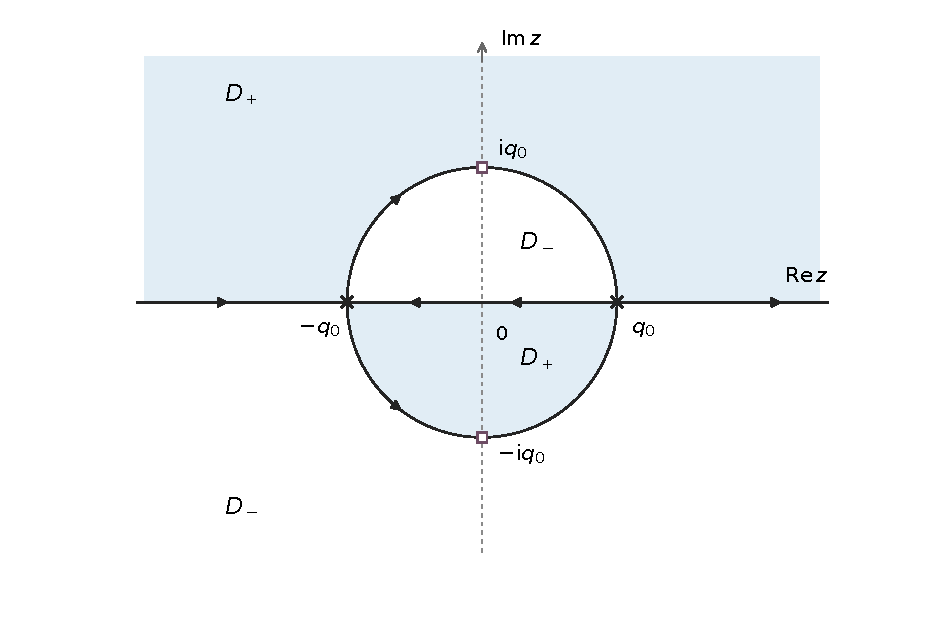
\includegraphics[width=0.78\textwidth]{figures/analytic-regions.pdf}
\caption{HMB 的单值化谱平面. 公共边界 $\Sigma$ 由实轴与圆 $|z|=q_0$ 组成; 淡蓝色区域为 $D_+$, 白色区域为 $D_-$. 箭头使 $D_+$ 位于定向边界的左侧. 方形点为分支点, 叉形点为边界交点.}
\label{fig:analytic-regions}
\end{figure}

为进行后续的轮廓积分, 将 $\Sigma$ 定向为 $D_+$ 位于左侧: 实轴外段朝右, 内段朝左, 上半圆顺时针, 下半圆逆时针. $z=\pm\ii q_0$ 为背景特征向量退化的分支点, $z=\pm q_0$ 为轮廓交点. 共振原像 $z_a^\pm$ 处空间谱问题正则; 其 Jost 值取固定 $t$ 的空间归一化.
